\documentclass[12pt, titlepage]{article}

% basics
\usepackage[utf8]{inputenc}

\usepackage{textcomp}
% \usepackage[dutch]{babel}
\usepackage{url}
% \usepackage{hyperref}
% \hypersetup{
%     colorlinks,
%     linkcolor={black},
%     citecolor={black},
%     urlcolor={blue!80!black}
% }
\usepackage{graphicx}
\usepackage{float}
\usepackage{booktabs}
\usepackage{enumitem}
% \usepackage{parskip}
\usepackage{emptypage}
\usepackage{subcaption}
\usepackage{multicol}
\usepackage[usenames,dvipsnames]{xcolor}

% \usepackage{cmbright}

\usepackage{amsmath, amsfonts, mathtools, amsthm, amssymb}
\usepackage{mathrsfs}
\usepackage{cancel}
\usepackage{bm}
\newcommand\N{\ensuremath{\mathbb{N}}}
\newcommand\R{\ensuremath{\mathbb{R}}}
\newcommand\Z{\ensuremath{\mathbb{Z}}}
\renewcommand\O{\ensuremath{\emptyset}}
\newcommand\Q{\ensuremath{\mathbb{Q}}}
\newcommand\C{\ensuremath{\mathbb{C}}}
\DeclareMathOperator{\sgn}{sgn}
\usepackage{systeme}
\let\svlim\lim\def\lim{\svlim\limits}
\let\implies\Rightarrow
\let\impliedby\Leftarrow
\let\iff\Leftrightarrow
\let\epsilon\varepsilon
\usepackage{stmaryrd} % for \lightning
\newcommand\contra{\scalebox{1.1}{$\lightning$}}
% \let\phi\varphi
% theorems
\makeatother
\usepackage{thmtools}
\usepackage[framemethod=TikZ]{mdframed}
\mdfsetup{skipabove=1em,skipbelow=0em}

\definecolor{geyecolor}{RGB}{199,237,204}%
\theoremstyle{definition}

\declaretheoremstyle[
    headfont=\bfseries\sffamily\color{ForestGreen!70!black}, 
    numbered=no,
    mdframed={
        linewidth=3pt,
        rightline=false, topline=false, bottomline=false,
        linecolor=ForestGreen, backgroundcolor=ForestGreen!1,
    }
]{thmgreenbox}

\declaretheoremstyle[
    headfont=\bfseries\sffamily\color{NavyBlue!70!black}, 
    numbered=no,
    mdframed={
        linewidth=2pt,
        rightline=false, topline=false, bottomline=false,
        linecolor=NavyBlue, backgroundcolor=NavyBlue!1,
    }
]{thmbluebox}

% Algoritmo.
\declaretheoremstyle[
    headfont=\bfseries\sffamily\color{OliveGreen!70!black}, 
    numbered=no,
    mdframed={
        linewidth=2pt,
        rightline=false, topline=false, bottomline=false,
        linecolor=OliveGreen, backgroundcolor=OliveGreen!1,
    }
]{thmorangealgo}

\declaretheoremstyle[
    headfont=\bfseries\sffamily\color{NavyBlue!70!black},
    numbered=no, 
    mdframed={
        linewidth=2pt,
        rightline=false, topline=false, bottomline=false,
        linecolor=NavyBlue
    }
]{thmblueline}

\declaretheoremstyle[
    headfont=\bfseries\sffamily\color{RawSienna!70!black}, 
    mdframed={
        linewidth=2pt,
        rightline=false, topline=false, bottomline=false,
        linecolor=RawSienna, backgroundcolor=RawSienna!1,
    }
]{thmredbox}

\declaretheoremstyle[
    headfont=\bfseries\sffamily\color{RawSienna!70!black}, 
    numbered=no,
    mdframed={
        linewidth=2pt,
        rightline=false, topline=false, bottomline=false,
        linecolor=RawSienna, backgroundcolor=RawSienna!1,
    },
]{thmproofbox}

\declaretheoremstyle[
    headfont=\bfseries\sffamily\color{NavyBlue!70!black}, 
    numbered=no,
    mdframed={
        linewidth=2pt,
        rightline=false, topline=false, bottomline=false,
        linecolor=NavyBlue, backgroundcolor=NavyBlue!1,
    },
]{thmexplanationbox}


\declaretheorem[style=thmgreenbox, numbered=no, name=Curve di apprendimento]{curve}
\declaretheorem[style=thmgreenbox, numbered=no, name=Risultati]{risultati}
\declaretheorem[style=thmbluebox, numbered=no, name=Feature Importance]{featimp}
\declaretheorem[style=thmbluebox, numbered=no, name=Esempio]{es}
\declaretheorem[style=thmbluebox, numbered=no, name=Iperparametri]{iperparametri}
\declaretheorem[style=thmredbox, numbered=no, name=Attenzione]{attenzione}
\declaretheorem[style=thmredbox, numbered=no, name=Interpretazione]{interpretazione}
\declaretheorem[style=thmredbox, name=Teorema]{theorem}
\declaretheorem[style=thmredbox, name=Esercizio]{esercizio}
\declaretheorem[style=thmorangealgo, name=Soluzione]{sol}
\declaretheorem[style=thmredbox, numbered=no, name=Lemma]{lemma}
\declaretheorem[style=thmredbox, numbered=no, name=Corollario]{corollary}
\declaretheorem[style=thmorangealgo, numbered=no, name=Algoritmo]{algo}

\declaretheorem[style=thmproofbox, name=Dimostrazione]{replacementproof}
\renewenvironment{proof}[1][\proofname]{\vspace{-10pt}\begin{replacementproof}}{\end{replacementproof}}


\declaretheorem[style=thmexplanationbox, name=Dimostrazione]{tmpexplanation}
\newenvironment{explanation}[1][]{\vspace{-10pt}\begin{tmpexplanation}}{\end{tmpexplanation}}

\declaretheorem[style=thmblueline, numbered=no, name=Ricorda]{remark}
\declaretheorem[style=thmblueline, numbered=no, name=Nota]{note}
\declaretheorem[style=thmblueline, numbered=no, name=Osservazione]{obs}

\newtheorem*{uovt}{UOVT}
\newtheorem*{notation}{Notation}
\newtheorem*{previouslyseen}{As previously seen}
\newtheorem*{problem}{Problem}
\newtheorem*{observe}{Observe}
\newtheorem*{property}{Property}
\newtheorem*{intuition}{Intuition}


\usepackage{etoolbox}
\AtEndEnvironment{vb}{\null\hfill$\diamond$}%
\AtEndEnvironment{intermezzo}{\null\hfill$\diamond$}%
% \AtEndEnvironment{opmerking}{\null\hfill$\diamond$}%

% http://tex.stackexchange.com/questions/22119/how-can-i-change-the-spacing-before-theorems-with-amsthm
\makeatletter
% \def\thm@space@setup{%
%   \thm@preskip=\parskip \thm@postskip=0pt
% }

\newcommand{\oefening}[1]{%
    \def\@oefening{#1}%
    \subsection*{Oefening #1}
}

\newcommand{\suboefening}[1]{%
    \subsubsection*{Oefening \@oefening.#1}
}

\newcommand{\exercise}[1]{%
    \def\@exercise{#1}%
    \subsection*{Exercise #1}
}

\newcommand{\subexercise}[1]{%
    \subsubsection*{Exercise \@exercise.#1}
}


\usepackage{xifthen}

\def\testdateparts#1{\dateparts#1\relax}
\def\dateparts#1 #2 #3 #4 #5\relax{
    \marginpar{\small\textsf{\mbox{#1 #2 #3 #5}}}
}

\def\@lesson{}%
\newcommand{\lesson}[3]{
    \ifthenelse{\isempty{#3}}{%
        \def\@lesson{Lecture #1}%
    }{%
        \def\@lesson{Lecture #1: #3}%
    }%
    \subsection*{\@lesson}
    \testdateparts{#2}
}

% \renewcommand\date[1]{\marginpar{#1}}


\usepackage[a4paper,width=165mm,top=20mm,bottom=20mm,bindingoffset=6mm]{geometry}
\usepackage[utf8]{inputenc}
\usepackage[italian]{babel}
\usepackage[OT1]{fontenc}
\usepackage{graphicx}
\usepackage{float}
\usepackage{fancyhdr}
\usepackage{xcolor}
\usepackage{mathtools}
\usepackage{amsmath}
\usepackage{amssymb}
\usepackage{tikz}
\usepackage{imakeidx}
\usepackage{textcomp}
\usepackage{pifont}
\usepackage{polynom}
\usepackage{algorithm}
\usepackage{algpseudocode}
\usepackage{mathtools}
\usepackage[colorlinks=true,linkcolor=black,anchorcolor=black,citecolor=black,filecolor=black,menucolor=black,runcolor=black,urlcolor=blue]{hyperref}
\usepackage{cancel}
\usepackage{pgfplots}
\usepackage{tabularx}

\colorlet{punct}{red!60!black}
\definecolor{background}{HTML}{EEEEEE}
\definecolor{delim}{RGB}{20,105,176}
\colorlet{numb}{magenta!60!black}
\pagestyle{fancy}
\everymath{\displaystyle}


%\cite{nome}



\begin{document}

  \bibliographystyle{plain} % We choose the "plain" reference style
  \begin{titlepage}
    \begin{center}
        
\includegraphics[width=0.4\textwidth]{img/logo_uniba}\\
        \vspace{1cm}
        % Dipartimento
        {\large Dipartimento di Informatica}\\
        \vspace{1cm}
        % Corso di laurea
        {\large Corso di laurea in Informatica}\\
        \hrulefill \\
        \vspace{2cm}
        {\large \textbf{Caso di Studio per l'esame di Ingegneria della Conoscenza}}\\
        \vspace{2cm}
        % Titolo
        {\LARGE\textbf{Sistema intelligente per l'assegnazione del Corporate Credit Rating alle aziende}}\\
        \vspace{2cm}

       \begin{table}[ht]
          \centering
          \begin{tabularx}{\textwidth}{@{}X@{}}
              Progetto di: \\
              \textbf{Mattia Curri} (758306) \href{mailto:m.curri8@studenti.uniba.it}{m.curri8@studenti.uniba.it} \\
          \end{tabularx}
      \end{table}
      \vspace{1cm}

      \begin{table}[ht]
        \centering
        \begin{tabularx}{\textwidth}{@{}X@{}}
            Link Repository: \\
            \href{https://github.com/mattiacurri/ProgettoICON}{https://github.com/mattiacurri/ProgettoICON} \\
        \end{tabularx}
    \end{table}

        \vspace{4cm}
        \hrulefill \\
        \vspace{1cm}
        % Anno accademico in cui si è iscritti
        {\large Anno Accademico \textbf{2023-2024}}
    \end{center}
\end{titlepage}
  \tableofcontents
  \newpage

  \section{Introduzione}

\noindent Nell'attuale panorama economico globale, le valutazioni delle aziende svolgono un ruolo cruciale nel determinare il loro status finanziario e creditizio. Le agenzie di rating forniscono valutazioni e raccomandazioni ai mercati finanziari, agli investitori e alle stesse aziende stesse, influenzando direttamente le decisioni di investimento e i flussi di capitale. In questo contesto, l'applicazione di tecniche di apprendimento supervisionato si presenta come un'opportunità significativa per migliorare e automatizzare il processo di valutazione aziendale.

\noindent Il progetto ha l'obiettivo di predire il Corporate Credit Rating, l'opinione di un'agenzia indipendente sulla probabilità che una società adempia pienamente ai propri obblighi finanziari alla scadenza.

\noindent Come riporta \cite{investopediacorporatecredit}, ogni agenzia ha un proprio sistema di rating, ma sono tutti simili. Ad esempio, Standard and Poor's utilizza "AAA" per la massima qualità del credito con il rischio di credito più basso, "AA" per la migliore, seguita da "A" e "BBB" per un credito soddisfacente. Questi rating sono considerati "investment grade", il che significa che la società valutata ha un livello di qualità richiesto da molte istituzioni. Tutto ciò che è inferiore a "BBB" è considerato speculativo o peggio, fino a un rating "D", che indica "spazzatura".

\noindent Il progetto utilizza i dati forniti e adottati da \cite{makwana2022get}, base di partenza per l'implementazione del sistema, a cui è stato integrato \cite{nguyen2021multimodal}, che utilizza un dataset differente e meno ricco di esempi, ma che comunque propone degli interessanti spunti di partenza per affrontare il problema.
Inoltre, \cite{makwana2022get} propone come sviluppo futuro quello di trattare il problema come un problema multiclasse invece che binario e di considerare più settori, cosa che è stata fatta in questo studio, seppure non tenendo conto delle date dei rating.
\subsection{Elenco argomenti di interesse}

\begin{itemize}[label=-]
    \item \textbf{Apprendimento Supervisionato} \cite{PooleMackworth23Ch7}: Valutare le Predizioni, Alberi di Decisione, Cross Validation, Modelli compositi: Boosting e Bagging, \textit{Oversampling, undersampling, tecniche miste, valutare le predizioni in presenza di sbilanciamento delle classi}
    \item \textbf{Apprendimento Probabilistico} \cite{PooleMackworth23Ch10}: Rete Bayesiana, Apprendimento della Struttura, Query, Generazione di nuovi Samples, \textit{Valutazione}
\end{itemize}
\noindent In \textit{corsivo} gli argomenti extra trattati.
  \newpage
  \section{Preprocessing dei dati}

\noindent Il dataset presenta le seguenti feature (in \textcolor{red}{rosso} la feature target):

\begin{itemize}[label=-]
    \item \textbf{Rating Agency}: l'agenzia di rating che ha assegnato il rating
    \item \textbf{Corporation}: la società valutata
    \item \textcolor{red}{\textbf{Rating}}: il rating assegnato
    \item \textbf{Rating Date}: la data in cui è stato assegnato il rating
    \item \textbf{CIK}: il CIK (Central Index Key) della società, ID univoco
    \item \textbf{Binary Rating}: il rating binario assegnato a seguito dello studio di \cite{makwana2022get}
    \item \textbf{Ticker}: il simbolo utilizzato per identificare la società in borsa
    \item \textbf{SIC Code}: codice utilizzato per classificare le attività economiche
    \item \textbf{Sector}: il settore di appartenenza della società, in \cite{makwana2022get} è stata valutata soltanto gli esempi con settore "BusEq" (Business Equipment), qui verranno utilizzati tutti
    \item \textbf{Current Ratio}: rapporto tra attività correnti e passività correnti
    \item \textbf{Long-term Debt / Capital}: rapporto tra debito a lungo termine e capitale
    \item \textbf{Debt Equity Ratio}: quanto un'azieda è propensa a chiedere prestiti invece di chiedere finanziamenti agli azionisti
    \item \textbf{Net Profit Margin}: margine di profitto netto
    \item \textbf{Gross Margin}: margine di profitto lordo
    \item \textbf{Operation Margin}: profito dopo aver coperto i costi di produzione
    \item \textbf{EBIT Margin}: profito prima delle tasse
    \item \textbf{Asset Turnover}: rapporto tra vendite e attività totali
    \item \textbf{EBITDA Margin}: profito prima delle tasse, ammortamenti e svalutazioni
    \item \textbf{Pre-Tax Profit Margin}: profito prima delle tasse
    \item \textbf{ROE - Return on Equity}: profito netto su capitale proprio, ovvero l'efficienza dei soldi investiti
    \item \textbf{ROA - Return on Assets}: profito netto su attività totali
    \item \textbf{ROI - Return on Investment}: profito netto su investimenti
    \item \textbf{Return On Tangible Equity}: profito netto su capitale proprio tangibile
    \item \textbf{Operating Cash Flow Per Share}: flusso di cassa operativo per azione
    \item \textbf{Free Cash Flow Per Share}: flusso di cassa libero per azione
\end{itemize}

\noindent Il dataset è stato preprocessato come segue. \\ Si è scelto di seguire la strada di \cite{makwana2022get}, ovvero quella di utilizzare un misto tra conoscenze di dominio e correlazione delle feature (utilizzando il coefficiente di Pearson) per ridurre il numero di feature. \\
Si è scelto di rimuovere le feature \textit{Rating Agency}, \textit{Corporation}, \textit{CIK}, \textit{Binary Rating}, \textit{Ticker}, \textit{SIC Code}, in quanto non rilevanti per il problema in esame. Sono stati rimossi anche \textbf{Corporation} e \textbf{Ticker} (non seguendo quindi la suddivisione di esperimenti di \cite{nguyen2021multimodal}): si è deciso di affrontare il problema indipendentemente dalla società ma soltanto con uno spaccato di una società rappresentata dai valori numerici, economici e settoriali. \textbf{Rating Date} è stato trasformato in \textbf{Year Month Day}, featuredalla forma \textit{YYYYMMDD}, in modo da poterlo utilizzare come feature numerica. E' stata poi applicata una tecnica di \textbf{one-hot encoding} sulle feature \textbf{Rating Agency}e \textbf{Sector}. \\ Per quanto rigurda \textbf{Rating}, il dataset presentava tutti i rating in formato testuale, pertanto si è deciso di mappare i rating a valori numerici. Prima di fare ciò, si è deciso di ridurre il numero di classi: per ogni valore di Rating, come ad esempio "A", una società può ricevere come rating sfaccettature come "A+" o "A-", risultando quindi in circa 22 classi. I dati a disposizione non permetterebbero di realizzare un modello che riesca a predire esattamente il rating di una società, pertanto si è deciso di ridurre il numero di classi a 5, mappando i rating come segue:
\begin{itemize}[label=-]
    \item \textbf{AAA} (Rischio minimo):  0
    \item \textbf{Da AA+ a A-} (Rischio basso):  0
    \item \textbf{BBB+, BBB, BBB-} (Rischio medio): 1
    \item \textbf{Da BB+ a B-} (Rischio alto): 2
    \item \textbf{Da CCC+ a C-} (Rischio molto alto): 3
    \item \textbf{D+, D, D-} (Default): 3
\end{itemize}
\noindent Il rischio molto alto e il default sono stati uniti, così come rischio minimo e rischio basso, per mancanza di dati per le classi più estreme. More on that later.
\\ Infine, è stata applicata una normalizzazione \textit{MinMaxScaler} ai dati numerici (escluse le colonne one-hot encoded e il rating), in modo da avere tutti i dati in un range compreso tra 0 e 1, tranne per \textbf{Asset Turnover} a cui è stata applicata la \textit{PowerTransformer} perchè presentava una distribuzione molto sbilanciata. \\ Il \textcolor{red}{\textbf{dataset finale}} è così composto:
\begin{itemize}[label=-]
    \item \textbf{Rating Agency}: l'agenzia di rating che ha assegnato il rating \textit{one-hot encoded}
    \item \textbf{Year Month Day}: la data in cui è stato assegnato il rating (con formato \textit{YYYYMMDD})
    \item \textbf{Current Ratio}: rapporto tra attività correnti e passività correnti (\textit{normalizzato})
    \item \textbf{Debt Equity Ratio}: quanto un'azieda è propensa a chiedere prestiti invece di chiedere finanziamenti agli azionisti (\textit{normalizzato})
    \item \textbf{Net Profit Margin}: margine di profitto netto (\textit{normalizzato})
    \item \textbf{Gross Margin}: margine di profitto lordo (\textit{normalizzato})
    \item \textbf{Asset Turnover}: rapporto tra vendite e attività totali (\textit{normalizzato})
    \item \textbf{EBITDA Margin}: profito prima delle tasse, ammortamenti e svalutazioni (\textit{normalizzato})
    \item \textbf{ROE - Return on Equity}: profito netto su capitale proprio, ovvero l'efficienza dei soldi investiti (\textit{normalizzato})
    \item \textbf{ROA - Return on Assets}: profito netto su attività totali (\textit{normalizzato})
    \item \textbf{ROI - Return on Investment}: profito netto su investimenti (\textit{normalizzato})
    \item \textbf{Return On Tangible Equity}: profito netto su capitale proprio tangibile (\textit{normalizzato})
    \item \textbf{Operating Cash Flow Per Share}: flusso di cassa operativo per azione (\textit{normalizzato})
    \item \textbf{Free Cash Flow Per Share}: flusso di cassa libero per azione (\textit{normalizzato})
    \item \textbf{Sector}: il settore di appartenenza della società (\textit{one-hot encoded})
\end{itemize}
\noindent Sono state quindi rimosse usando come discriminante il dominio \textit{Long-term Debt / Capital}, \textit{Operation Margin}, \textit{Pre-Tax Profit Margin} e \textit{EBIT Margin}. \\ A questo punto, dando un'occhiata ai dati, possiamo notare un netto sbilanciamento delle classi, in particolare quella di rischio altissimo.
\begin{figure}[H]
    \centering
    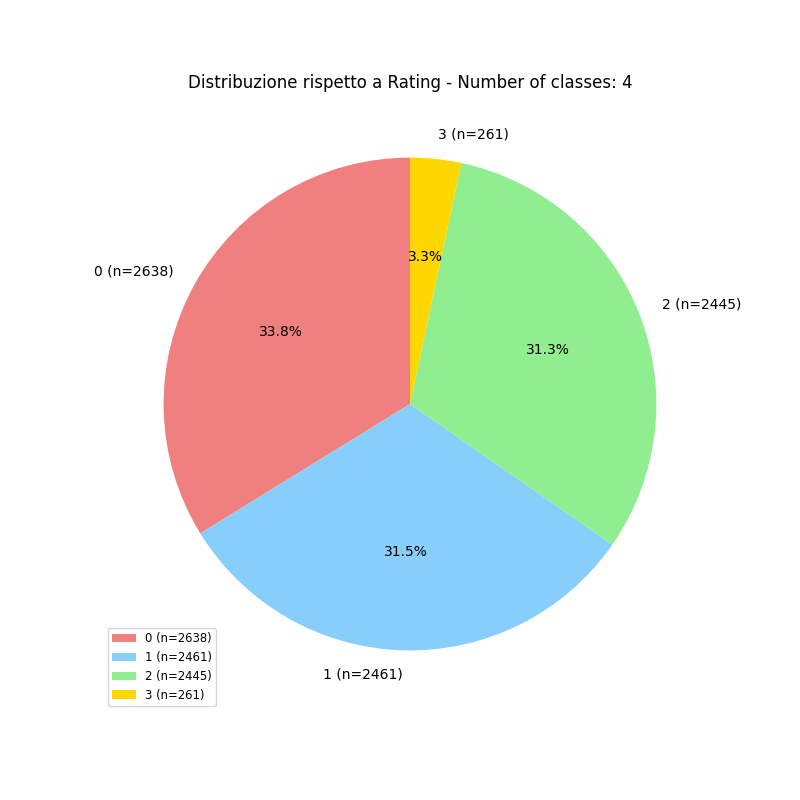
\includegraphics[scale=0.5]{img/class_imbalance.png}
\end{figure}
\noindent Pertanto, quello che stiamo per affrontare è un problema di classificazione multiclasse sbilanciato.
  \newpage
  \section{Apprendimento Supervisionato}

\subsection{Modelli e metodologie utilizzate}

\paragraph{Modelli adottati.} Per qusto progetto ho deciso di adottare principalmente quattro modelli di apprendimento automatico:
\begin{itemize}[label=-]
    \item \textbf{Decision Tree}: classificatore strutturato ad albero in cui le foglie
    rappresentano le classi di appartenenza (o le probabilità di appartenenza a tali
    classi) mentre la radice e i nodi interni rappresentano delle condizioni sulle
    feature di input. A seconda se tali condizioni sono rispettate o meno, verrà
    seguito un percorso piuttosto che un altro e alla fine si arriverà alla classe di
    appartenenza
    \item \textbf{RandomForest}: classificatore che si ottiene creando tanti DecisionTree. Il valore in output si ottiene mediando sulle predizioni di ogni albero
    appartenente alla foresta (tecnica di bagging)
    \item \textbf{XGBoost}: utilizza un approccio di boosting basato sul gradiente che combina diverse versioni di alberi decisionali deboli per creare un modello complessivo più potente
    \item \textbf{LightGBM}: altra libreria di boosting basata sul gradiente progettata per massimizzare l'efficienza computazionale. Si distingue per la sua velocità di addestramento e di previsione, grazie all'utilizzo di un algoritmo di divisione foglia-per-foglia e ad altre ottimizzazioni che minimizzano la memoria e la computazione necessarie.
\end{itemize}
\noindent Si è scelto di non usare modelli come ad esempio la regressione logistica, in quanto il rating può non essere direttamente correlato con le features a nostra disposizione (a titolo di esempio \cite{ilfattoquotidiano}), e quindi la linearità del modello non si presta bene. In alcuni esperimenti alcuni di questi sono stati scartati o sostituiti, in tal caso verrà specificato nella sezione apposita.
\paragraph{Train Test Split.} Per valutare le performance dei modelli, si è diviso il dataset in due parti: una parte per l'addestramento e una parte per la validazione. Si è scelto di adottare una divisione 80-20 \textbf{stratificata}, in modo da mantenere la stessa distribuzione delle classi nel training set e nel test set.
\paragraph{Cross-Validation.} Per trovare i migliori iperparametri per ogni modello, e per la fase di valutazione si è adottata una \textit{Repeated Stratified K-fold cross validation}, in cui la cross validation viene ripetuta per $m$ volte mantenendo nei fold la distribuzione originaria delle classi. Il numero \textit{K} di fold è stato definito per ogni esperimento dalla regola di Sturges, una delle regole empiriche per la scelta del numero di classi in un istogramma. La regola di Sturges suggerisce di utilizzare un numero di classi pari a $1 + \log_2(n)$, dove $n$ è il numero di osservazioni. In questo caso, per garantire un numero di fold non troppo elevato mantenendo comunque la regola, si è scelto di adottare la regola usando la seguente formula: $\dfrac{1 + \log_2(n)}{3}$.
\paragraph{Ricerca degli iperparametri.} Per la ricerca degli iperparametri migliori si è adottata una \textit{GridSearchCV} con una \textit{Repeated Stratified K-fold Cross-Validation}. Di seguito la descrizione degli iperparametri per ogni modello e i valori testati:
% TODO
\begin{itemize}[label=-]
    \item \textbf{Decision Tree}: \textit{max\_depth} (massima profondità dell'albero), \textit{min\_samples\_split} (numero minimo di campioni necessari per suddividere un nodo interno), \textit{min\_samples\_leaf} (numero minimo di campioni necessari per essere in una foglia), \textit{max\_features} (numero di feature da considerare per la migliore suddivisione), \textit{criterion} (funzione per misurare la qualità di una suddivisione)
    \item \textbf{RandomForest}: \textit{n\_estimators} (numero di alberi nella foresta), \textit{max\_depth}
    \item \textbf{XGBoost}: \textit{n\_estimators}, \textit{max\_depth}, \textit{learning\_rate}, \textit{subsample}, \textit{colsample\_bytree}
    \item \textbf{LightGBM}: \textit{n\_estimators}, \textit{max\_depth}, \textit{learning\_rate}, \textit{subsample}, \textit{colsample\_bytree}
\end{itemize}
\paragraph{Riproducibilità.} Per garantire la riproducibilità dei risultati, si è scelto di fissare il \textit{seed} per la generazione di numeri casuali al numero \textit{42}.
\paragraph{Valutazione.} La parte di valutazione è stata fatta utilizzando una \textit{cross\_val\_score}, ovvero un metodo che valuta sempre utilizzando la Cross Validation i modelli addestrati. Per la valutazione delle performance del sistema ho deciso di utilizzare le seguenti metriche:
\begin{itemize}[label=-]
    \item \textbf{Balanced Accuracy}: È una versione modificata dell'accuratezza standard che tiene conto dello sbilanciamento delle classi nei dati. Calcola la media delle accuratezze per ciascuna classe, fornendo quindi una valutazione equilibrata delle prestazioni del modello su tutte le classi. Utilizzare un'accuracy normale sarebbe fuorviante, dato che potrebbe bastare al classificatore predire sempre le classi più frequenti per ottenere un'accuracy alta
    \item \textbf{Cohen's Kappa}: è una misura della concordanza tra le predizioni di un classificatore e i veri valori delle classi, correggendo l'accordo che potrebbe verificarsi solo per caso. Questa metrica tiene conto dell'equilibrio tra le classi e fornisce una valutazione più accurata rispetto alla semplice accuratezza. Il valore di Cohen's Kappa varia da -1 a 1, dove 1 indica una perfetta concordanza tra le predizioni e i veri valori, 0 indica concordanza casuale e valori negativi indicano concordanza peggiore di quella casuale
    \item \textbf{Geometric Mean}: è la radice del prodotto della sensibilità per classe. Questa misura cerca di massimizzare l'accuratezza su ciascuna delle classi, mantenendo queste accuratezze bilanciate. Per i problemi multiclasse è la radice n-esima del prodotto della sensibilità per ciascuna classe. Se almeno una classe non viene riconosciuta dal classificatore, la geometric mean sarà 0, pertanto ci servirà per dare soprattutto un \textit{lower bound} di confronto per i nostri modelli.
\end{itemize}
\noindent La \textit{GridSearchCV} è stata allenata nel trovare gli iperparametri che massimizzano la \textit{Balanced accuracy}. Sono state poi prese in considerazione \textbf{varianza} e \textbf{deviazione standard} per ogni modello: un modello con una varianza e una deviazione standard più basse è preferibile, in quanto indica che le predizioni sono più coerenti e affidabili.

\subsection{Primo esperimento}
\noindent Nel primo esperimento si è provato ad allenare i modelli proposti in precedenza sugli esempi del dataset senza alcuna manipolazione successiva a quelle raccontate in precedenza. Sono state utilizzate le metriche e i modelli proposti in precedenza.

\paragraph{Iperparametri.} Di seguito si riportano gli iperparametri ottenuti dalla \textit{GridSearchCV} per ogni modello:
    
        
        \begin{table}[H]
            \centering
            \begin{tabular}{|l|l|}
            \hline
            \textbf{Parametro}                 & \textbf{Valore} \\ \hline
            LightGBM\_\_learning\_rate            & 0.1             \\ \hline
            LightGBM\_\_max\_depth                & 10              \\ \hline
            LightGBM\_\_n\_estimators             & 200             \\ \hline
            LightGBM\_\_lambda                    & 0.1             \\ \hline
            LightGBM\_\_num\_leaves               & 15              \\ \hline
            LightGBM\_\_min\_gain\_to\_split      & 0.1             \\ \hline
            LightGBM\_\_verbose                   & 0               \\ \hline
            XGBoost\_\_learning\_rate         & 0.1             \\ \hline
            XGBoost\_\_max\_depth             & 10              \\ \hline
            XGBoost\_\_n\_estimators          & 100             \\ \hline
            XGBoost\_\_lambda                 & 0.1             \\ \hline
            DecisionTree\_\_criterion         & log\_loss       \\ \hline
            DecisionTree\_\_max\_depth        & 40              \\ \hline
            DecisionTree\_\_min\_samples\_split & 5               \\ \hline
            DecisionTree\_\_min\_samples\_leaf & 2               \\ \hline
            RandomForest\_\_n\_estimators     & 100             \\ \hline
            RandomForest\_\_max\_depth        & 20              \\ \hline
            RandomForest\_\_min\_samples\_split & 2               \\ \hline
            RandomForest\_\_min\_samples\_leaf & 2               \\ \hline
            RandomForest\_\_criterion         & log\_loss       \\ \hline
            \end{tabular}
            \caption{Parametri del modello}
            
            \end{table}
\paragraph{Risultati.} Di seguito si riportano i risultati ottenuti per ogni metrica e per ogni modello:
\begin{figure}[H]
    \centering
    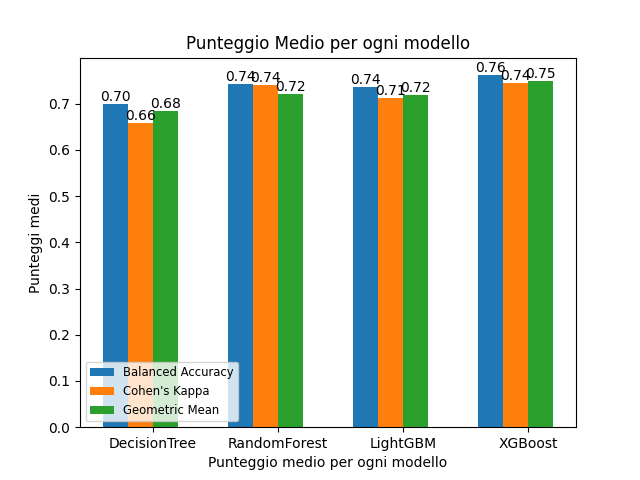
\includegraphics[scale=0.5]{img/normal_metrics.png}
\end{figure}
\noindent I primi risultati sono incoraggianti, soprattutto per i modelli basati su boosting e bagging, un pò meno per il decision tree. Le metriche non ci danno informazioni particolarmente utili riguardante un possibile overfitting o underfitting, però ci fanno capire come già di base i modelli si comportano abbastanza bene.

\paragraph{Curve di apprendimento.} Di seguito si riportano le curve di apprendimento per ogni modello, con tanto di deviazione standard e varianza:

\begin{figure}[H]
    \centering
    \begin{minipage}[b]{0.45\linewidth}
      \centering
      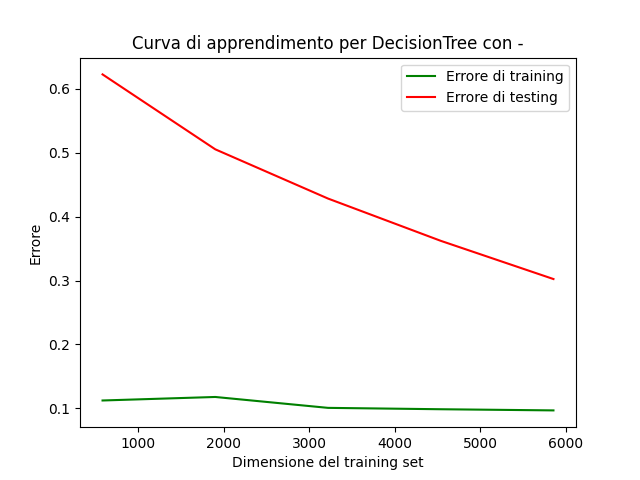
\includegraphics[scale=0.5]{img/learning_curve_DecisionTree_-.png}
      
    \end{minipage}
    \hfill
    \begin{minipage}[b]{0.45\linewidth}
      \centering
      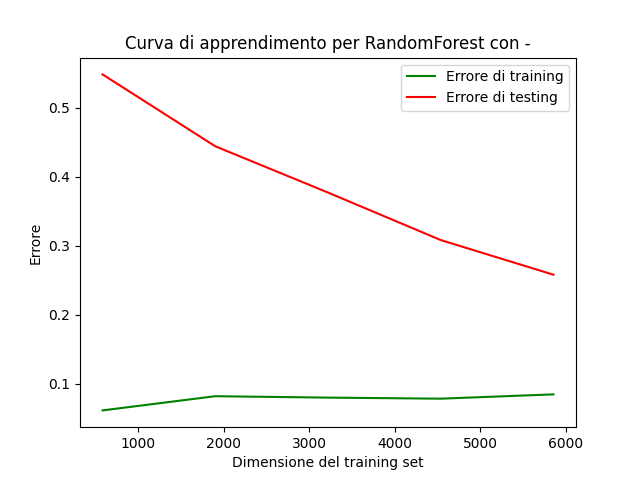
\includegraphics[scale=0.5]{img/learning_curve_RandomForest_-.png}
      
    \end{minipage}
    
    \begin{minipage}[b]{0.45\linewidth}
      \centering
      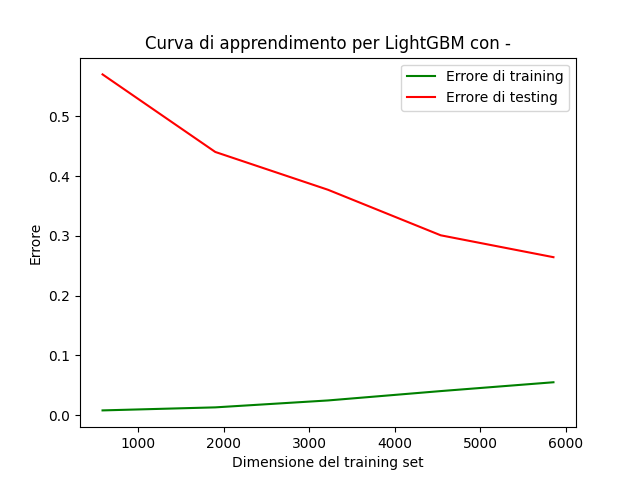
\includegraphics[scale=0.5]{img/learning_curve_LightGBM_-.png}
      
    \end{minipage}
    \hfill
    \begin{minipage}[b]{0.45\linewidth}
      \centering
      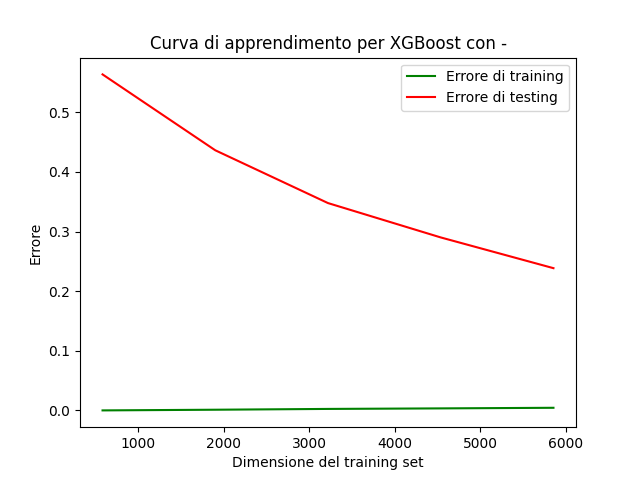
\includegraphics[scale=0.5]{img/learning_curve_XGBoost_-.png}
      
    \end{minipage}
    \caption{Curve di apprendimento.}
    
    \end{figure}

\begin{table}[H]
    \centering
    \begin{tabular}{lcc}
    \toprule
    \textbf{Modello} & \textbf{Train Error Std} & \textbf{Test Error Std} \\
    \midrule
    LightGBM & 0.003677832760964418 & 0.014729799395024678 \\
    XGBoost & 0.0017806001233474666 & 0.014258802458827638 \\
    DecisionTree & 0.004798633588628468 & 0.015296962637326389 \\
    RandomForest & 0.004364244206597904 & 0.014128073154668751 \\
    \bottomrule
    \end{tabular}
    \caption{Errori Standard per i Modelli}
    
\end{table}

\begin{table}[H]
    \centering
    \begin{tabular}{lcc}
    \toprule
    \textbf{Modello} & \textbf{Train Error Var} & \textbf{Test Error Var} \\
    \midrule
    LightGBM & 1.3526453817623153e-05 & 0.00021696699021766939 \\
    XGBoost & 3.1705367992650135e-06 & 0.00020331344755986913 \\
    DecisionTree & 2.3026884317913326e-05 & 0.0002339970659277595 \\
    RandomForest & 1.9046627494823375e-05 & 0.00019960245106367185 \\
    \bottomrule
    \end{tabular}
    \caption{Varianza degli Errori per i Modelli}
    
\end{table}

\noindent Il \textbf{Decision Tree} non sembra dare segni di overfitting quanto quasi più di underfitting, dato che l'errore di training si stabilizza dopo circa metà training set, ma l'errore di testing è ancora in discesa ed è un pò lontano dall'errore di traning. Il \textbf{Random Forest} presenta un piccolo picco nell'errore di training dopo circa 2000 esempi, stessa cosa dopo altri 2000, ma comunque sono picchi poco significativi, anche qui l'errore di testing è abbastanza lontano, quindi non si può parlare di overfitting. Il \textbf{LightGBM} mostra dei possibili primi segnali di overfitting: l'errore di training inizia ad aumentare col tempo, l'errore di testing inizia a scendere abbastanza velocemente. L'\textbf{XGBoost} non presenta problemi, riesce ad essere allenato senza problemi, ma l'errore di testing è comunque ancora abbastanza alto, quindi non si può parlare di overfitting. In conclusione, i modelli non presentano segni di overfitting, ma il LightGBM potrebbe presentare dei segni di overfitting in futuro.

\paragraph{Feature importances.} E' stata raccolta anche l'informazione riguardo quali feature abbiano contribuito di più in ogni modello per le predizioni.
\\Questo è stato fatto nel primo esperimento, in modo da utilizzare le feature maggiormente predittive per i modelli considerati migliori per costruire la rete bayesiana. Si riporta di seguito solo il grafico relativo al Random Forest, per non appesantire la trattazione, gli altri sono disponibili nel repository:

\begin{figure}[H]
    \centering
    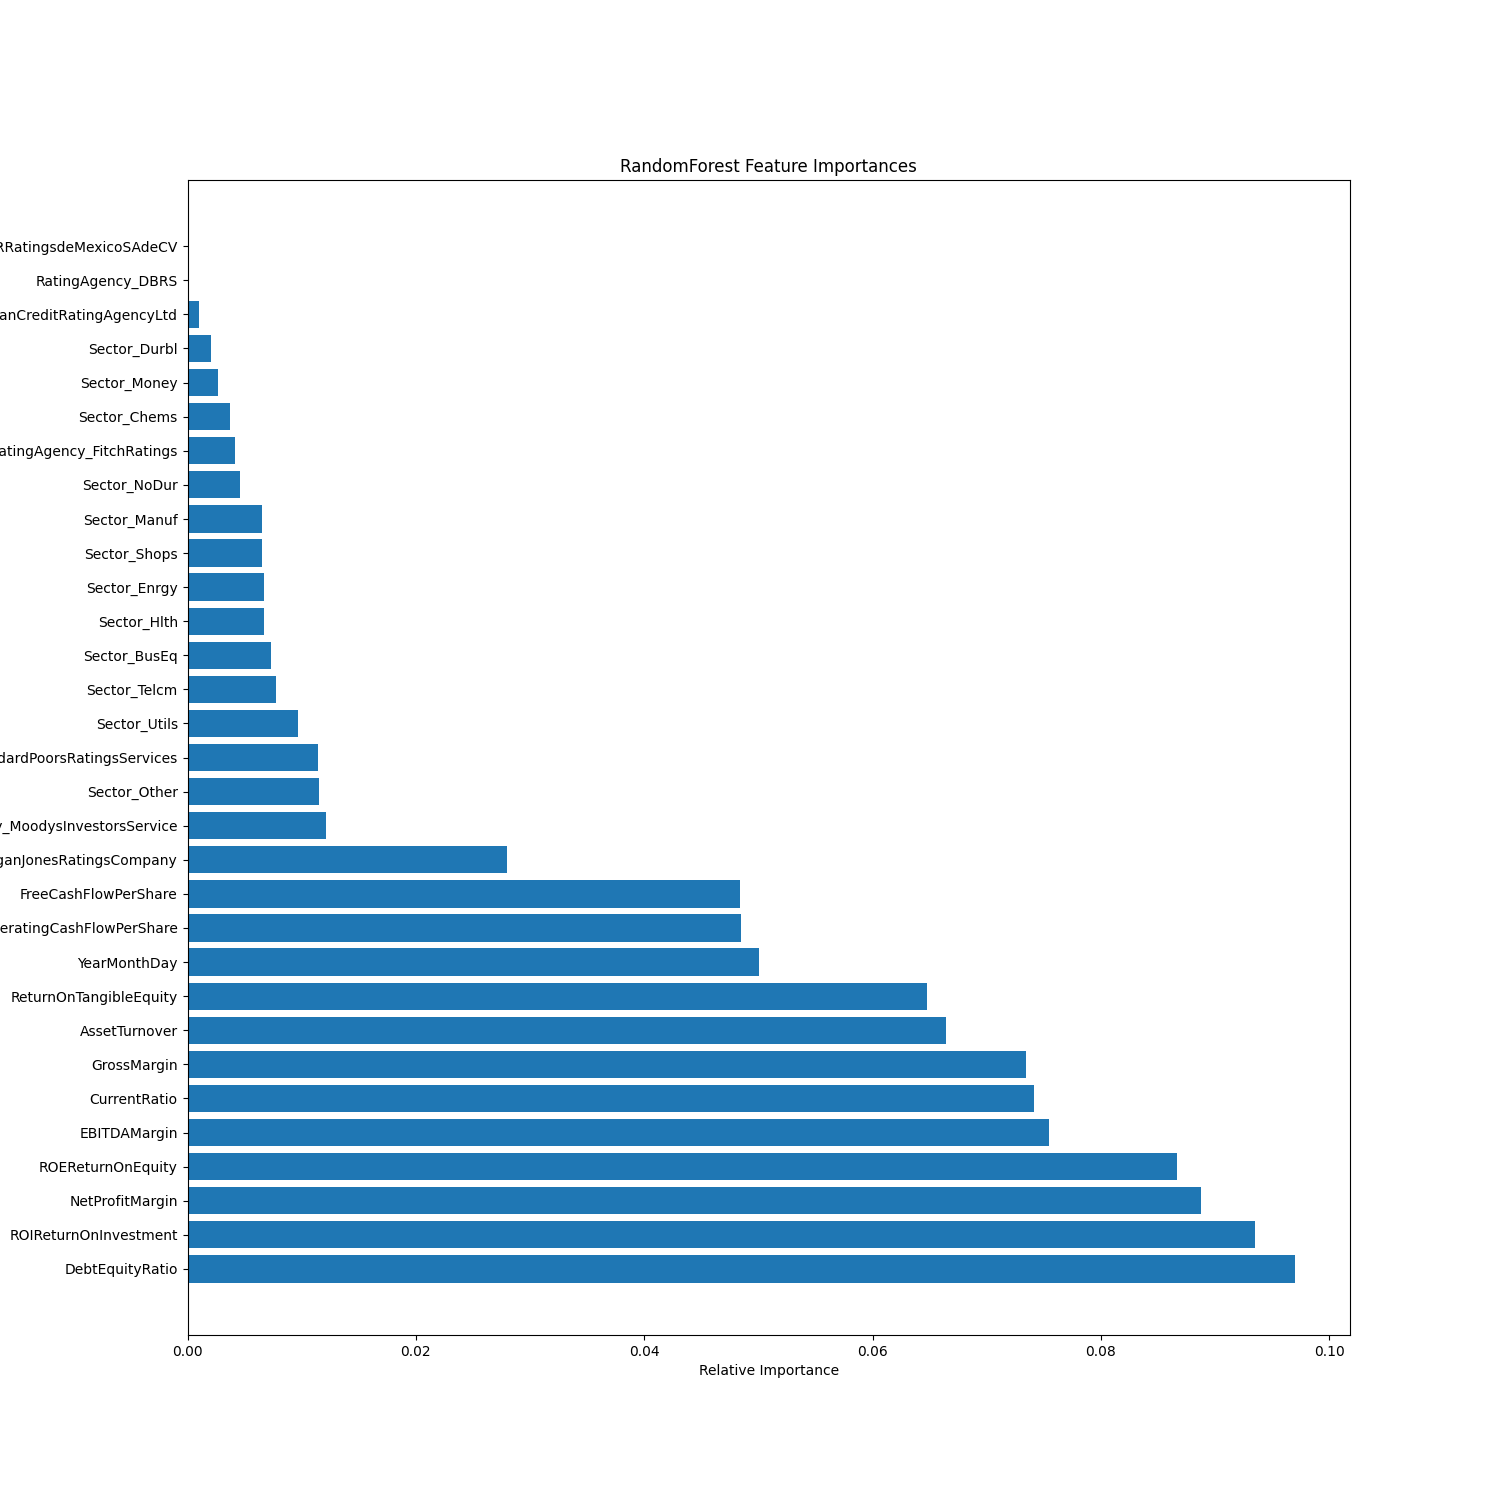
\includegraphics[scale=0.35]{img/feature_importances_RandomForest.png}
\end{figure}


\subsection{Secondo esperimento: class weights vs BalancedRF}
\noindent La tecnica del class weight assegna pesi differenti alle classi durante il processo di addestramento del modello. In particolare, si attribuiscono pesi maggiori alle classi minoritarie e pesi minori alle classi maggioritarie. Questo consente al modello di dare maggiore importanza alle istanze delle classi minoritarie durante l'addestramento, venendo penalizzato meno per gli errori commessi su queste classi. In questo modo, il modello sarà in grado di apprendere meglio le caratteristiche delle classi minoritarie e di migliorare le prestazioni su queste classi.\\
I pesi delle classi possono essere calcolati in diversi modi. Uno dei metodi comuni è utilizzare l'inverso della frequenza delle classi nel dataset, che è la tecnica che andremo ad utilizzare.\\ \\ Per questo esperimento, andremo a usare tre modelli, tagliando fuori l'XGBoost, in quanto non supporta nativamente la possibilità di assegnare un peso alle classi.\\ In alternativa si utilizzerà un \textit{BalancedRandomForest}, che si differenzia dal classico \textit{Random Forest} per il fatto che estrarrà un campione su cui allenare ogni singolo \textit{decision tree} dalla classe di minoranza e campionerà con sostituzione lo stesso numero di campioni dalla classe di maggioranza. E' un modello che si presta bene proprio per classificazione con classi sbilanciate, pertanto lo testeremo contro dei modelli impostati con un \textbf{bias} verso le classi minoritarie.

\paragraph{Iperparametri.} Per il BalancedRandomForest lo spazio di ricerca degli iperparametri scelto è il medesimo dei Random Forest. Di seguito si riportano gli iperparametri ottenuti dalla \textit{GridSearchCV} per ogni modello:

\begin{table}[H]
\centering
\begin{tabular}{|l|l|}
\toprule
\textbf{Parametro}                 & \textbf{Valore} \\ \midrule
BalancedRandomForest\_\_criterion & entropy \\ 
BalancedRandomForest\_\_n\_estimators & 200 \\
BalancedRandomForest\_\_max\_depth & 20 \\
BalancedRandomForest\_\_min\_samples\_split & 2 \\
BalancedRandomForest\_\_min\_samples\_leaf & 2 \\
BalancedRandomForest\_\_sampling\_strategy & all \\
BalancedRandomForest\_\_replacement & True \\
LightGBM\_\_learning\_rate & 0.1 \\
LightGBM\_\_max\_depth & 10 \\
LightGBM\_\_n\_estimators & 200 \\
LightGBM\_\_lambda & 0.5 \\
LightGBM\_\_num\_leaves & 15 \\
LightGBM\_\_min\_gain\_to\_split & 0.1 \\
LightGBM\_\_verbose & 0 \\
LightGBM\_\_class\_weight & balanced \\
DecisionTree\_\_criterion & entropy \\
DecisionTree\_\_max\_depth & 40 \\
DecisionTree\_\_min\_samples\_split & 2 \\
DecisionTree\_\_min\_samples\_leaf & 2 \\
DecisionTree\_\_class\_weight & balanced \\
RandomForest\_\_n\_estimators & 200 \\
RandomForest\_\_max\_depth & 20 \\
RandomForest\_\_min\_samples\_split & 10 \\
RandomForest\_\_min\_samples\_leaf & 2 \\
RandomForest\_\_criterion & log\_loss \\
RandomForest\_\_class\_weight & balanced \\ \bottomrule
\end{tabular}
\caption{Parametri del modello}
\end{table}

\paragraph{Risultati.} Di seguito si riportano i risultati ottenuti per ogni metrica e per ogni modello:

\begin{figure}[H]
    \centering
    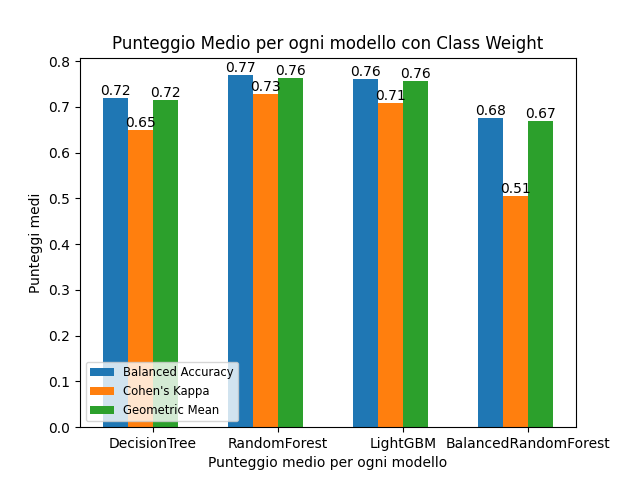
\includegraphics[scale=0.7]{img/cw_metrics.png}
\end{figure}

\noindent A un primo impatto possiamo vedere come il BalancedRandomForest non è riuscito a mantenere le aspettative, soprattutto se confrontato con il suo "gemello", il Random Forest classico. Rispetto al primo esperimento, le metriche di tutti gli altri modelli sono leggermente migliorati, ma siamo molto vicini ai range di varianza e deviazione standard del primo esperimento.\\

\paragraph{Curve di apprendimento.} Di seguito si riportano le curve di apprendimento per ogni modello, con tanto di deviazione standard e varianza:

\begin{figure}[H]
    \centering
    \begin{minipage}[b]{0.45\linewidth}
      \centering
      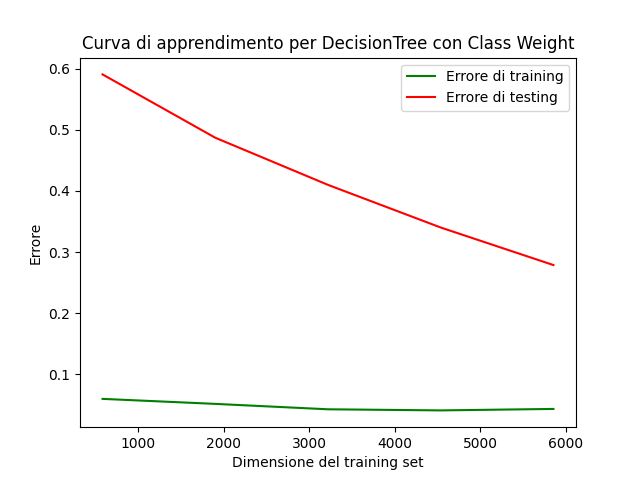
\includegraphics[scale=0.5]{img/learning_curve_DecisionTree_Class Weight.png}
      
    \end{minipage}
    \hfill
    \begin{minipage}[b]{0.45\linewidth}
      \centering
      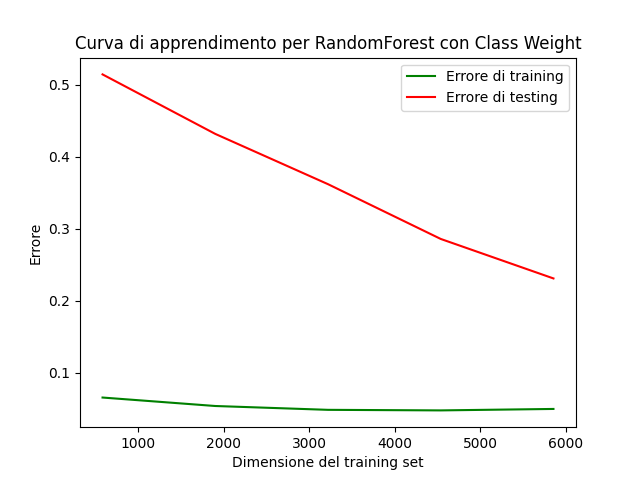
\includegraphics[scale=0.5]{img/learning_curve_RandomForest_Class Weight.png}
      
    \end{minipage}
    
    \begin{minipage}[b]{0.45\linewidth}
      \centering
      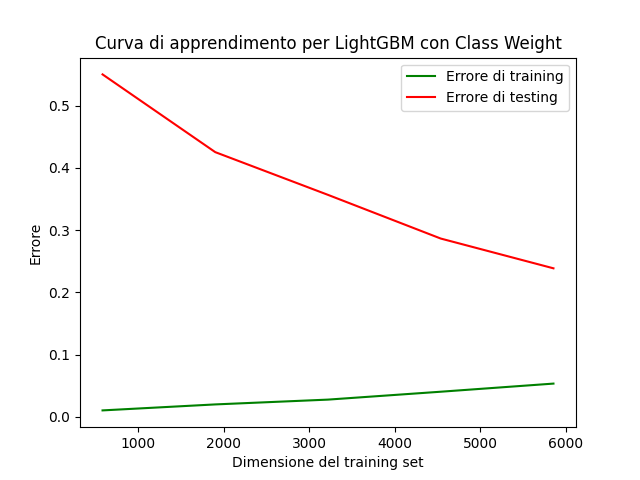
\includegraphics[scale=0.5]{img/learning_curve_LightGBM_Class Weight.png}
      
    \end{minipage}
    \hfill
    \begin{minipage}[b]{0.45\linewidth}
      \centering
      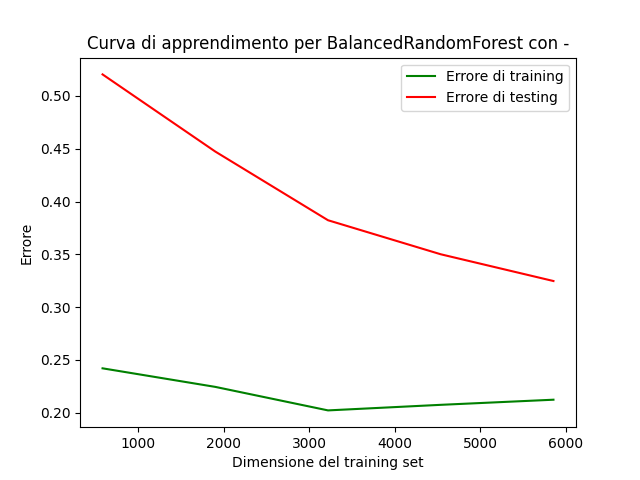
\includegraphics[scale=0.5]{img/learning_curve_BalancedRandomForest_-.png}
      
    \end{minipage}
    \caption{Curve di apprendimento.}
    
    \end{figure}

\begin{table}[H]
    \centering
    \begin{tabular}{lcc}
    \toprule
    \textbf{Modello} & \textbf{Train Error Std} & \textbf{Test Error Std} \\
    \midrule
    LightGBM & 0.0026561375826418482 & 0.016525860583798364 \\
    BalancedRandomForest & 0.004339002154983959 & 0.009953134681109565\\
    DecisionTree & 0.0015879855371825314 & 0.015329002342180082 \\
    RandomForest & 0.0018445912002196091 & 0.02129919916812779 \\
    \bottomrule
    \end{tabular}
    \caption{Errori Standard per i Modelli}
\end{table}


\begin{table}[H]
    \centering
    \begin{tabular}{lcc}
    \toprule
    \textbf{Modello} & \textbf{Train Error Var} & \textbf{Test Error Var} \\
    \midrule
    LightGBM & 7.055066857922481e-06 & 0.0002731040680351404 \\
    BalancedRandomForest & 1.8826939700955435e-05 & 9.906488998030602e-05 \\
    DecisionTree & 2.5216980663008927e-06 & 0.00023497831280656247 \\
    RandomForest & 3.4025166959276185e-06 & 0.00045365588520357555 \\
    \bottomrule
    \end{tabular}
    \caption{Varianza degli Errori per i Modelli}
\end{table}

\noindent Rispetto al primo esperimento il Decision Tree sembra essersi stabilizzato ancora di più, il Random Forest presenta un errore di training decisamente più lineare, il LightGBM non presenta miglioramenti.


\subsection{Terzo esperimento: oversampling}
\noindent L'oversampling consiste nell'aumentare artificialmente il numero di esempi delle classi minoritarie nel dataset di addestramento, in modo da bilanciare meglio la distribuzione delle classi. Ciò viene fatto replicando casualmente le istanze esistenti della classe minoritaria o generando nuove istanze sintetiche utilizzando tecniche come lo SMOTE, che testeremo. \\SMOTE sintetizza nuove istanze per la classe minoritaria creando campioni artificiali lungo le linee che collegano istanze simili nello spazio delle feature. In questo modo, si cerca di mantenere la struttura dei dati originari mentre si aumenta il numero di istanze della classe minoritaria. \\ Andremo a confrontare lo SMOTE con i risultati degli altri esperimenti e con quelli dell'ADASYN, un'altra tecnica di oversampling.\\ ADASYN genera nuovi esempi per le istanze delle classi minoritarie che hanno un alto grado di disomogeneità, ovvero che sono il più possibile differenti dagli esempi della classe maggioritaria per caratteristiche. Questa tecnica a differenza della precedente non riesce a garantire il perfetto ribilanciamento del dataset, ma ad ogni modo riesce quasi del tutto a risanarlo tranne nei casi in cui gli esempi della classe minoritaria sono sparsi e immersi in esempi di classe maggioritaria. \\ Gli algoritmi sono stati utilizzati con 
\textit{random\_state} uguale a \textit{42}, e con \textit{sampling\_strategy} uguale a \textit{all}, in modo da ribilanciare tutte le classi. Come sviluppo futuro si potrebbe pensare di fare una sorta di \textit{GridSearchCV} per trovare il miglior set di parametri per queste tecniche.
\begin{attenzione}
Si è prestata particolare attenzione nell'applicazione delle tecniche descritte nel seguito del capitolo. Infatti un errore comune è quello di utilizzare tecniche di oversampling, undersampling o miste su tutto il dataset, andando quindi ad allenare il modello sui dati sintetici, ma anche ad usare un test set con dati sintetici, che non rispecchia la realtà. Per questo motivo, si applicano le tecniche di oversampling soltanto sul training set, e non sul test set. Questo potrebbe portare a miglioramenti che non risultano entusiasmanti, ma è comunque la scelta migliore per valutare i nostri modelli.
\end{attenzione}

\subsubsection{SMOTE}
\paragraph{Iperparametri.} Di seguito si riportano gli iperparametri ottenuti dalla \textit{GridSearchCV} per ogni modello:

\begin{table}[H]
    \centering
    \begin{tabular}{|l|l|}
    \toprule
    \textbf{Parametro}                 & \textbf{Valore} \\ \midrule
    LightGBM\_\_learning\_rate            & 0.1             \\ 
    LightGBM\_\_max\_depth                & 10              \\ 
    LightGBM\_\_n\_estimators             & 200             \\ 
    LightGBM\_\_lambda                    & 0.01            \\ 
    LightGBM\_\_num\_leaves               & 15              \\ 
    LightGBM\_\_min\_gain\_to\_split      & 0.1             \\ 
    XGBoost\_\_learning\_rate         & 0.1             \\ 
    XGBoost\_\_max\_depth             & 10              \\ 
    XGBoost\_\_n\_estimators          & 100             \\ 
    XGBoost\_\_lambda                 & 0.01            \\ 
    DecisionTree\_\_criterion         & gini            \\ 
    DecisionTree\_\_max\_depth        & 20              \\ 
    DecisionTree\_\_min\_samples\_split & 5               \\ 
    DecisionTree\_\_min\_samples\_leaf & 2               \\ 
    RandomForest\_\_n\_estimators     & 200             \\ 
    RandomForest\_\_max\_depth        & 20              \\ 
    RandomForest\_\_min\_samples\_split & 2               \\ 
    RandomForest\_\_min\_samples\_leaf & 2               \\ 
    RandomForest\_\_criterion         & entropy         \\ \bottomrule
    \end{tabular}
    \caption{Parametri del modello}
    \end{table}

\paragraph{Risultati.} Di seguito si riportano i risultati ottenuti per ogni metrica e per ogni modello:

\begin{figure}[H]
    \centering
    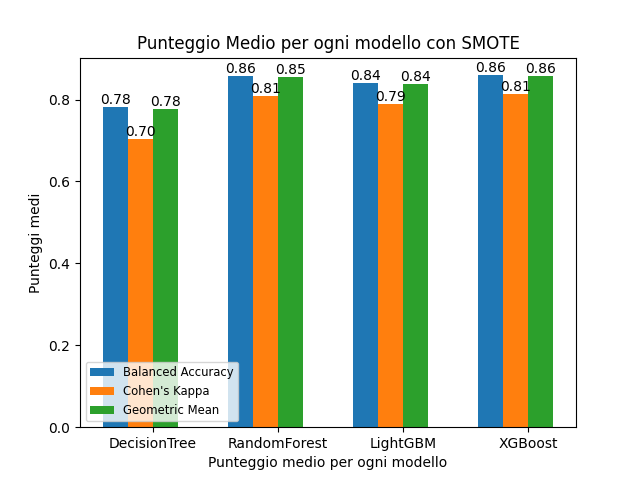
\includegraphics[scale=0.7]{img/smote_metrics.png}
\end{figure}

\noindent I risultati sono decisamente migliori rispetto ai due esperimenti precedenti, pertanto resta da controllare se vi è overfitting in qualche modello.

\paragraph{Curve di apprendimento.} Di seguito si riportano le curve di apprendimento per ogni modello, con tanto di deviazione standard e varianza:

\begin{figure}[H]
    \centering
    \begin{minipage}[b]{0.45\linewidth}
      \centering
      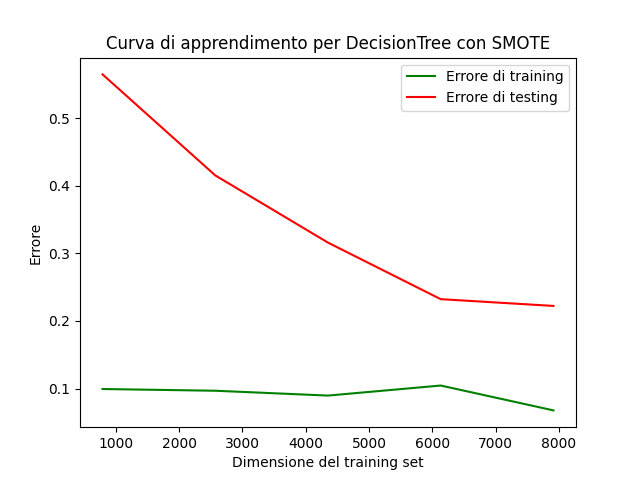
\includegraphics[scale=0.5]{img/learning_curve_DecisionTree_SMOTE.png}
      
    \end{minipage}
    \hfill
    \begin{minipage}[b]{0.45\linewidth}
      \centering
      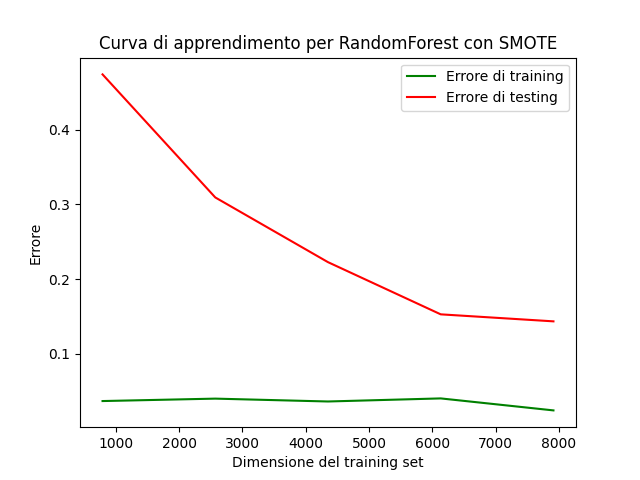
\includegraphics[scale=0.5]{img/learning_curve_RandomForest_SMOTE.png}
      
    \end{minipage}
    
    \begin{minipage}[b]{0.45\linewidth}
      \centering
      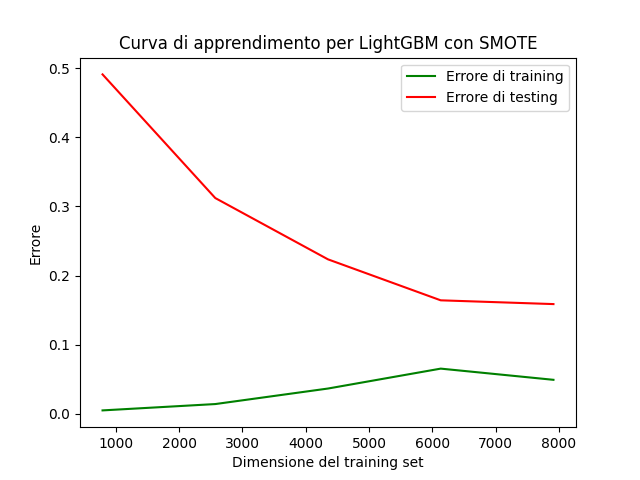
\includegraphics[scale=0.5]{img/learning_curve_LightGBM_SMOTE.png}
      
    \end{minipage}
    \hfill
    \begin{minipage}[b]{0.45\linewidth}
      \centering
      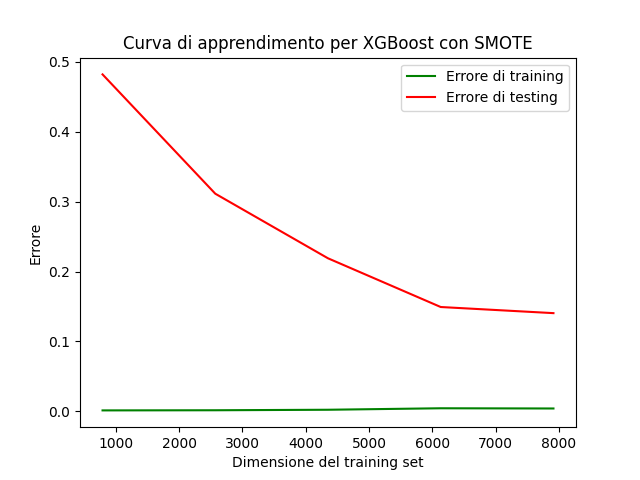
\includegraphics[scale=0.5]{img/learning_curve_XGBoost_SMOTE.png}
      
    \end{minipage}
    \caption{Curve di apprendimento.}
    
    \end{figure}

\begin{table}[H]
    \centering
    \begin{tabular}{lcc}
    \toprule
    \textbf{Modello} & \textbf{Train Error Std} & \textbf{Test Error Std} \\
    \midrule
    LightGBM & 0.0013274976900467363 & 0.005557462071090911 \\
    XGBoost & 0.0010996943494845943 & 0.007626860052066837 \\
    DecisionTree & 0.005071533109955392 & 0.006148834960506031 \\
    RandomForest & 0.000739498264938402 & 0.004926394385656445 \\
    \bottomrule
    \end{tabular}
    \caption{Errori Standard per i Modelli}
\end{table}

\begin{table}[H]
    \centering
    \begin{tabular}{lcc}
    \toprule
    \textbf{Modello} & \textbf{Train Error Var} & \textbf{Test Error Var} \\
    \midrule
    LightGBM & 1.7622501170794206e-06 & 3.088538467161408e-05 \\
    XGBoost & 1.209327662288345e-06 & 5.816899425381296e-05 \\
    DecisionTree & 2.5720448085373803e-05 & 3.7808171371541206e-05 \\
    RandomForest & 5.468576838469069e-07 & 2.426936164302734e-05 \\
    \bottomrule
    \end{tabular}
    \caption{Varianza degli Errori per i Modelli}
\end{table}
\noindent I valori di deviazione standard e varianza non portano a pensare a overfitting. Guardando le curve notiamo come l'XGBoost si sia comportato bene, stessa cosa per il Random Forest, mentre sorgono dubbi sull'efficacia del Decision Tree e del LightGBM, in particolare quest'ultimo sembra raggiungere una configurazione ideale tra i 6000 e gli 8000 esempi.

\subsubsection{ADASYN}
\paragraph{Iperparametri.} Di seguito si riportano gli iperparametri ottenuti dalla \textit{GridSearchCV} per ogni modello:

\begin{table}[H]
    \centering
    \begin{tabular}{|l|l|}
    \toprule
    \textbf{Parametro}                 & \textbf{Valore} \\ \midrule
    LightGBM\_\_learning\_rate            & 0.1             \\ 
    LightGBM\_\_max\_depth                & 10              \\ 
    LightGBM\_\_n\_estimators             & 200             \\ 
    LightGBM\_\_lambda                    & 0.1             \\ 
    LightGBM\_\_num\_leaves               & 15              \\ 
    LightGBM\_\_min\_gain\_to\_split      & 0.1             \\ 
    XGBoost\_\_learning\_rate         & 0.1             \\ 
    XGBoost\_\_max\_depth             & 20              \\ 
    XGBoost\_\_n\_estimators          & 100             \\ 
    XGBoost\_\_lambda                 & 0.01            \\ 
    DecisionTree\_\_criterion         & gini            \\ 
    DecisionTree\_\_max\_depth        & 40              \\ 
    DecisionTree\_\_min\_samples\_split & 5               \\ 
    DecisionTree\_\_min\_samples\_leaf & 2               \\ 
    RandomForest\_\_n\_estimators     & 200             \\ 
    RandomForest\_\_max\_depth        & 20              \\ 
    RandomForest\_\_min\_samples\_split & 2               \\ 
    RandomForest\_\_min\_samples\_leaf & 2               \\ 
    RandomForest\_\_criterion         & log\_loss         \\ \bottomrule
    \end{tabular}
    \caption{Parametri del modello}
    \end{table}

\paragraph{Risultati.} Di seguito si riportano i risultati ottenuti per ogni metrica e per ogni modello:

\begin{figure}[H]
    \centering
    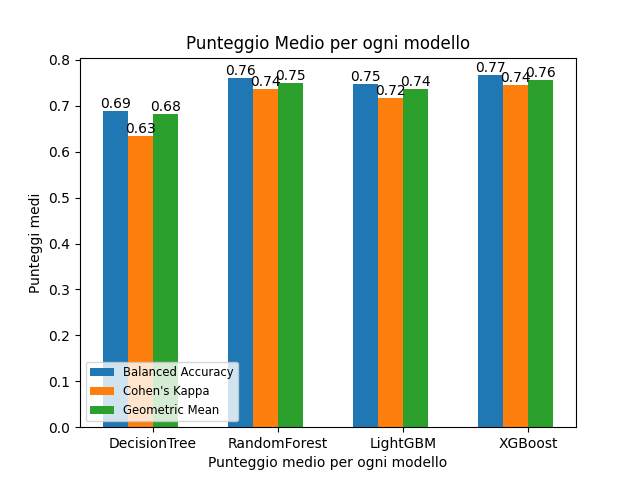
\includegraphics[scale=0.7]{img/adasyn_metrics.png}
\end{figure}

\noindent I punteggi sono simili agli esperimenti precedenti, ma non migliori dello SMOTE.

\paragraph{Curve di apprendimento.} Di seguito si riportano le curve di apprendimento per ogni modello, con tanto di deviazione standard e varianza:

\begin{figure}[H]
    \centering
    \begin{minipage}[b]{0.45\linewidth}
      \centering
      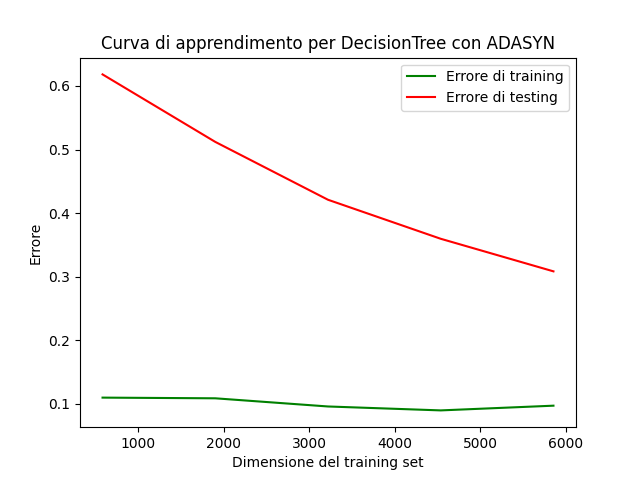
\includegraphics[scale=0.5]{img/learning_curve_DecisionTree_ADASYN.png}
      
    \end{minipage}
    \hfill
    \begin{minipage}[b]{0.45\linewidth}
      \centering
      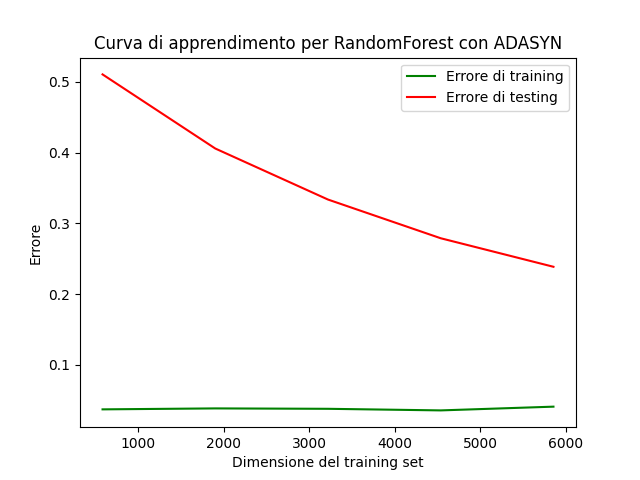
\includegraphics[scale=0.5]{img/learning_curve_RandomForest_ADASYN.png}
      
    \end{minipage}
    
    \begin{minipage}[b]{0.45\linewidth}
      \centering
      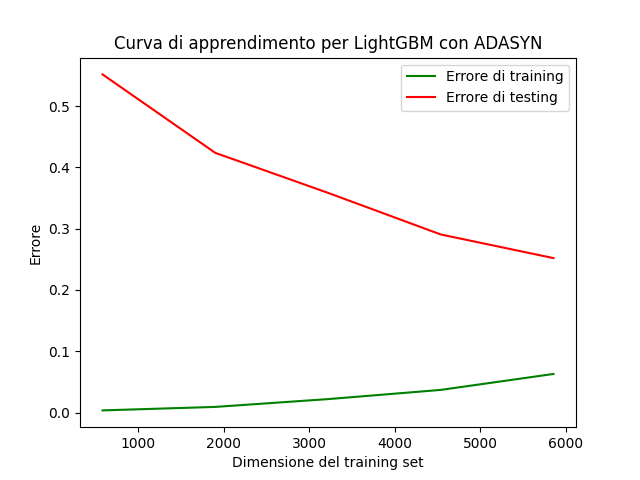
\includegraphics[scale=0.5]{img/learning_curve_LightGBM_ADASYN.png}
      
    \end{minipage}
    \hfill
    \begin{minipage}[b]{0.45\linewidth}
      \centering
      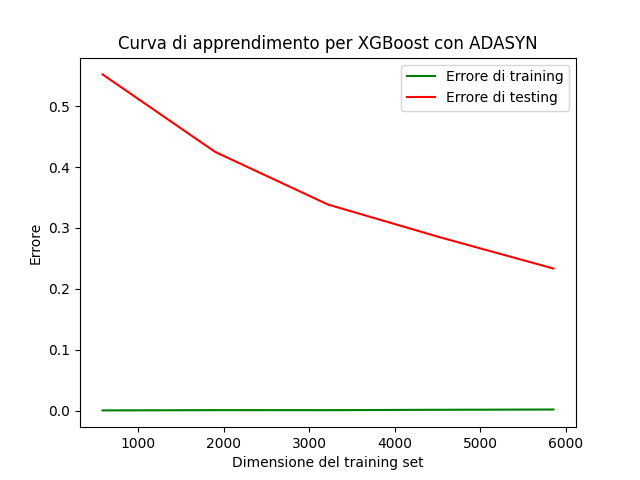
\includegraphics[scale=0.5]{img/learning_curve_XGBoost_ADASYN.png}
      
    \end{minipage}
    \caption{Curve di apprendimento.}
    
    \end{figure}

\begin{table}[H]
    \centering
    \begin{tabular}{lcc}
    \toprule
    \textbf{Modello} & \textbf{Train Error Std} & \textbf{Test Error Std} \\
    \midrule
    LightGBM & 0.0038361336791755867 & 0.014834571234512225 \\
    XGBoost & 0.0010135798069650331 & 0.01775432088891302 \\
    DecisionTree & 0.0050366494920735345 & 0.02674348515555034 \\
    RandomForest & 0.0028043557998990395 & 0.01884405548317221 \\
    \bottomrule
    \end{tabular}
    \caption{Errori Standard per i Modelli}
    
\end{table}

\begin{table}[H]
    \centering
    \begin{tabular}{lcc}
    \toprule
    \textbf{Modello} & \textbf{Train Error Var} & \textbf{Test Error Var} \\
    \midrule
    LightGBM & 1.4715921604505222e-05 & 0.00022006450371181758 \\
    XGBoost & 1.0273440250872736e-06 & 0.00031521591022649323 \\
    DecisionTree & 2.5367838106004596e-05 & 0.0007152139982651415\\
    RandomForest & 7.86441145242738e-06 & 0.00035509842705287254 \\
    \bottomrule
    \end{tabular}
    \caption{Varianza degli Errori per i Modelli}
    
\end{table}

\noindent Random Forest e XGBoost risultano molto stabili, l'XGBoost sembra avere avere varianza e deviazione standard migliori, mentre LightGBM ancora una volta è in difficoltà. Il Decision Tree si comporta benino, ma risultando comunque il peggiore tra i modelli.


\subsection{Quarto esperimento: tecniche miste}
\noindent Non si è fatto uso di tecniche di undersampling, ovvero di tecniche che riducono il numero di esempi della classe maggioritaria, in quanto dopo un tentativo con un algoritmo di questo tipo i risultati erano imprensentabili, portando a scartare del tutto questa tecnica. In alternativa si proverà a utilizzare delle tecniche miste di oversampling e undersampling: SMOTEEEN e SMOTETomek, tecniche che applicano prima lo SMOTE per fare oversampling, per poi "pulire" il dataset, rimuovendo \textit{noise} e osservazioni "troppo facili da classificare", con tecniche di undersampling (EEN e Tomek)\\ Tomek rimuove quegli esempi di classi differenti che sono molto vicini tra loro, poichè saranno difficili da classificare e non aiutano l'algoritmo a trovare una discriminante. \\ EEN rimuove gli esempi di classe maggioritaria che sono molto vicini a quelli di classe minoritaria o gli esempidove tutti o quasi i vicini sono di classi differenti, poichè potrebbero essere classificati erroneamente.

\subsubsection{SMOTETomek}
\paragraph{Iperparametri.} Di seguito si riportano gli iperparametri ottenuti dalla \textit{GridSearchCV} per ogni modello:

\begin{table}[H]
    \centering
    \begin{tabular}{|l|l|}
    \toprule
    \textbf{Parametro}                 & \textbf{Valore} \\ \midrule
    LightGBM\_\_learning\_rate            & 0.1             \\ 
    LightGBM\_\_max\_depth                & 10              \\ 
    LightGBM\_\_n\_estimators             & 200             \\ 
    LightGBM\_\_lambda                    & 0.01            \\ 
    LightGBM\_\_num\_leaves               & 15              \\ 
    LightGBM\_\_min\_gain\_to\_split      & 0.1             \\ 
    XGBoost\_\_learning\_rate         & 0.1             \\ 
    XGBoost\_\_max\_depth             & 10              \\ 
    XGBoost\_\_n\_estimators          & 100             \\ 
    XGBoost\_\_lambda                 & 0.01            \\ 
    DecisionTree\_\_criterion         & gini            \\ 
    DecisionTree\_\_max\_depth        & 20              \\ 
    DecisionTree\_\_min\_samples\_split & 2               \\ 
    DecisionTree\_\_min\_samples\_leaf & 2               \\ 
    RandomForest\_\_n\_estimators     & 200             \\ 
    RandomForest\_\_max\_depth        & 20              \\ 
    RandomForest\_\_min\_samples\_split & 2               \\ 
    RandomForest\_\_min\_samples\_leaf & 2               \\ 
    RandomForest\_\_criterion         & log\_loss       \\ \bottomrule
    \end{tabular}
    \caption{Parametri del modello}
    
    \end{table}

\paragraph{Risultati.} Di seguito si riportano i risultati ottenuti per ogni metrica e per ogni modello:
\begin{figure}[H]
    \centering
    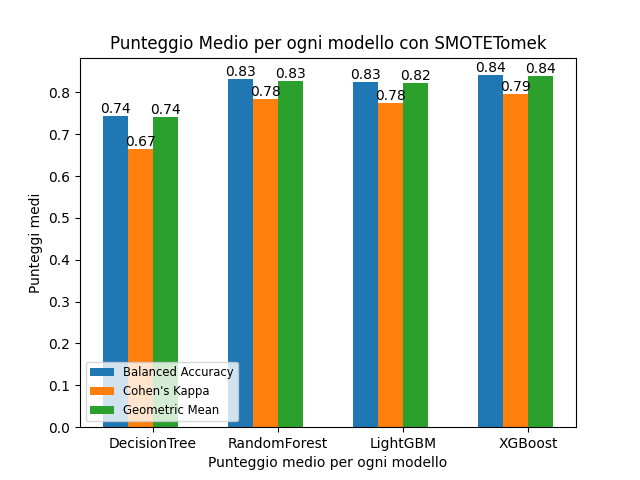
\includegraphics[scale=0.5]{img/tomek_metrics.png}
\end{figure}

\noindent I risultati sono simili all'esperimento con SMOTE. Verifichiamo se vi è overfitting.

\paragraph{Curve di apprendimento.} Di seguito si riportano le curve di apprendimento per ogni modello, con tanto di deviazione standard e varianza:

\begin{figure}[H]
    \centering
    \begin{minipage}[b]{0.45\linewidth}
      \centering
      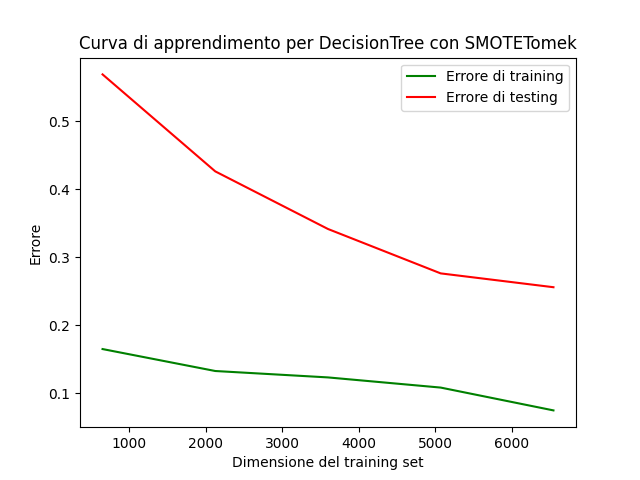
\includegraphics[scale=0.5]{img/learning_curve_DecisionTree_SMOTETomek.png}
      
    \end{minipage}
    \hfill
    \begin{minipage}[b]{0.45\linewidth}
      \centering
      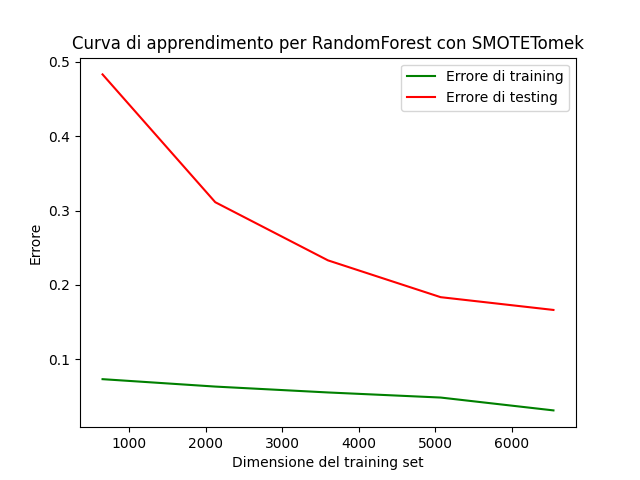
\includegraphics[scale=0.5]{img/learning_curve_RandomForest_SMOTETomek.png}
      
    \end{minipage}
    
    \begin{minipage}[b]{0.45\linewidth}
      \centering
      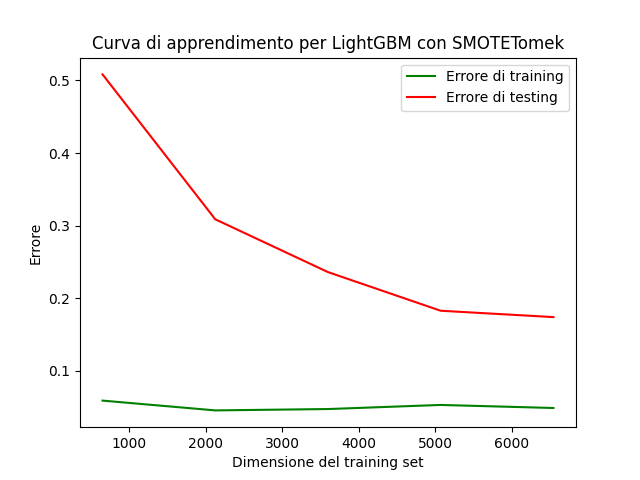
\includegraphics[scale=0.5]{img/learning_curve_LightGBM_SMOTETomek.png}
      
    \end{minipage}
    \hfill
    \begin{minipage}[b]{0.45\linewidth}
      \centering
      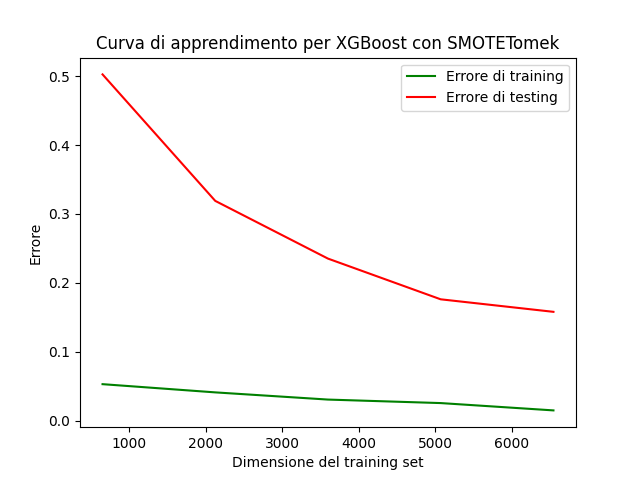
\includegraphics[scale=0.5]{img/learning_curve_XGBoost_SMOTETomek.png}
      
    \end{minipage}
    \caption{Curve di apprendimento.}
    
    \end{figure}

\begin{table}[H]
    \centering
    \begin{tabular}{lcc}
    \toprule
    \textbf{Modello} & \textbf{Train Error Std} & \textbf{Test Error Std} \\
    \midrule
    LightGBM & 0.0023555215150484524 & 0.009308465169567823 \\
    XGBoost & 0.0007603005596334415 & 0.007147550348338646 \\
    DecisionTree & 0.004106118784835311 & 0.010978248717168952 \\
    RandomForest & 0.001156335935796055 & 0.005023366391826634 \\
    \bottomrule
    \end{tabular}
    \caption{Errori Standard per i Modelli}
    
\end{table}

\begin{table}[H]
    \centering
    \begin{tabular}{lcc}
    \toprule
    \textbf{Modello} & \textbf{Train Error Var} & \textbf{Test Error Var} \\
    \midrule
    LightGBM & 5.548481607856157e-06 & 8.664752381305731e-05 \\
    XGBoost & 5.780569409789242e-07 & 5.1087475982035904e-05 \\
    DecisionTree & 1.6860211475177415e-05 & 0.00012052194489602173 \\
    RandomForest & 1.3371127964133382e-06 & 2.523420990653334e-05 \\
    \bottomrule
    \end{tabular}
    \caption{Varianza degli Errori per i Modelli}
    
\end{table}

\noindent Varianza e deviazione standard sono nella maggior parte dei casi maggiori rispetto all'esperimento con SMOTE e in generale i modelli sembrano aver bisogno di più dati per apprendere, notiamo come l'errore di training non si stabilizza in nessuno dei modelli.

\subsubsection{SMOTEENN}
\paragraph{Iperparametri.} Di seguito si riportano gli iperparametri ottenuti dalla \textit{GridSearchCV} per ogni modello:

\begin{table}[H]
    \centering
    \begin{tabular}{|l|l|}
    \toprule
    \textbf{Parametro}                 & \textbf{Valore} \\ \midrule
    LightGBM\_\_learning\_rate            & 0.05            \\ 
    LightGBM\_\_max\_depth                & 5               \\ 
    LightGBM\_\_n\_estimators             & 200             \\ 
    LightGBM\_\_lambda                    & 0.1             \\ 
    LightGBM\_\_num\_leaves               & 15              \\ 
    LightGBM\_\_min\_gain\_to\_split      & 0.1             \\ 
    XGBoost\_\_learning\_rate         & 0.1             \\ 
    XGBoost\_\_max\_depth             & 20              \\ 
    XGBoost\_\_n\_estimators          & 100             \\ 
    XGBoost\_\_lambda                 & 0.1             \\ 
    DecisionTree\_\_criterion         & log\_loss       \\ 
    DecisionTree\_\_max\_depth        & 40              \\ 
    DecisionTree\_\_min\_samples\_split & 2               \\ 
    DecisionTree\_\_min\_samples\_leaf & 2               \\ 
    RandomForest\_\_n\_estimators     & 100             \\ 
    RandomForest\_\_max\_depth        & 20              \\ 
    RandomForest\_\_min\_samples\_split & 2               \\ 
    RandomForest\_\_min\_samples\_leaf & 2               \\ 
    RandomForest\_\_criterion         & gini            \\ \bottomrule
    \end{tabular}
    \caption{Parametri del modello}
    
    \end{table}

\paragraph{Risultati.} Di seguito si riportano i risultati ottenuti per ogni metrica e per ogni modello:

\begin{figure}[H]
    \centering
    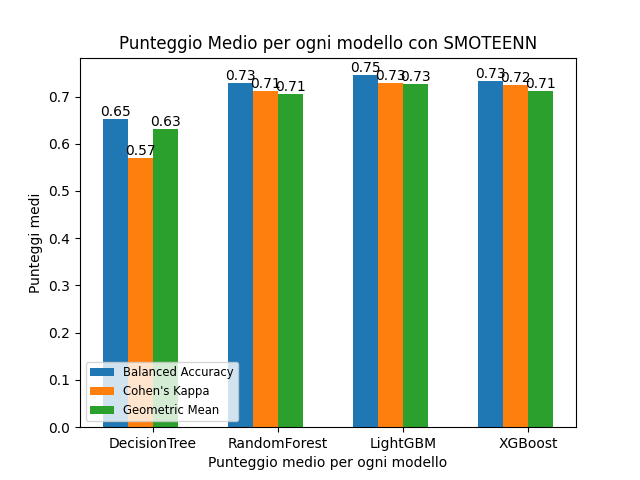
\includegraphics[scale=0.7]{img/smoteen_metrics.png}
\end{figure}

\noindent I risultati sono al pari dei primi esperimenti, se non inferiori.

\paragraph{Curve di apprendimento.} Di seguito si riportano le curve di apprendimento per ogni modello, con tanto di deviazione standard e varianza:

\begin{figure}[H]
    \centering
    \begin{minipage}[b]{0.45\linewidth}
      \centering
      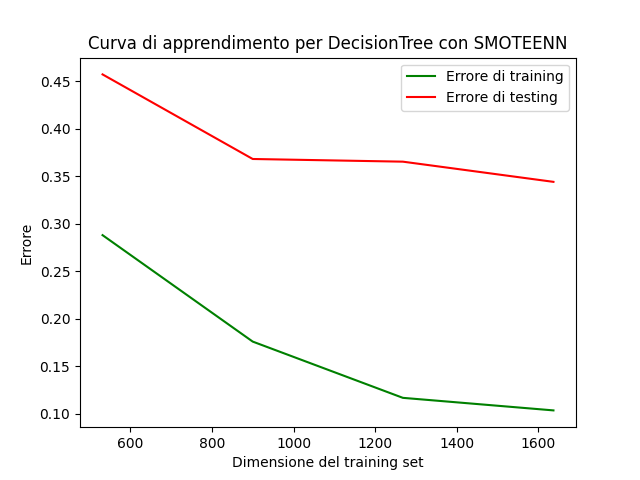
\includegraphics[scale=0.5]{img/learning_curve_DecisionTree_SMOTEENN.png}
      
    \end{minipage}
    \hfill
    \begin{minipage}[b]{0.45\linewidth}
      \centering
      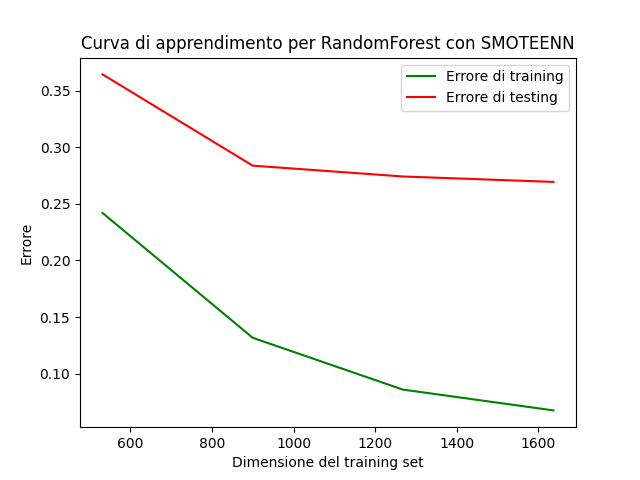
\includegraphics[scale=0.5]{img/learning_curve_RandomForest_SMOTEENN.png}
      
    \end{minipage}
    
    \begin{minipage}[b]{0.45\linewidth}
      \centering
      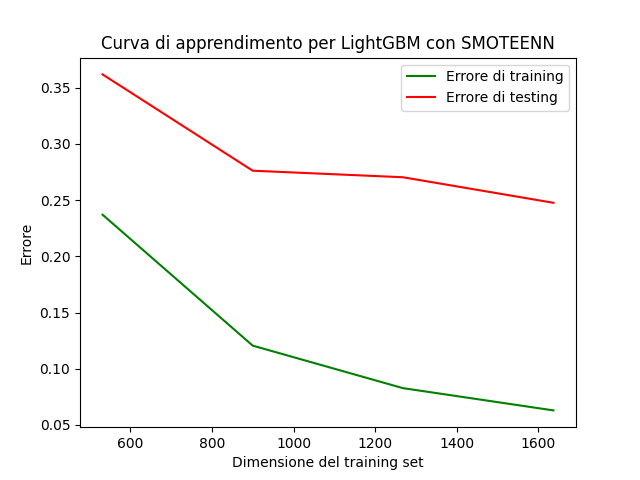
\includegraphics[scale=0.5]{img/learning_curve_LightGBM_SMOTEENN.png}
      
    \end{minipage}
    \hfill
    \begin{minipage}[b]{0.45\linewidth}
      \centering
      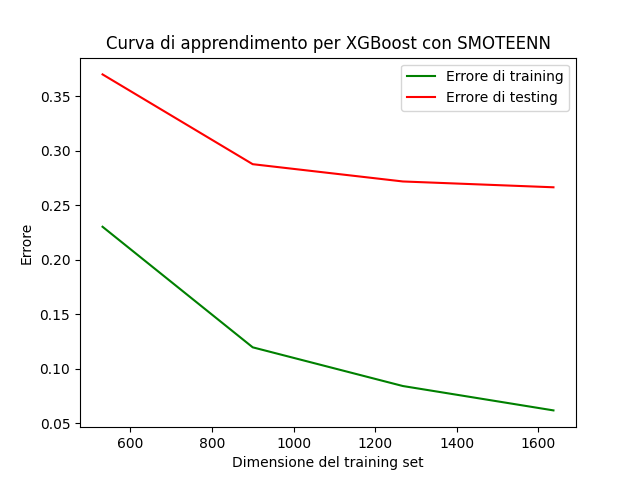
\includegraphics[scale=0.5]{img/learning_curve_XGBoost_SMOTEENN.png}
      
    \end{minipage}
    \caption{Curve di apprendimento.}
    
    \end{figure}


\begin{table}[H]
    \centering
    \begin{tabular}{lcc}
    \toprule
    \textbf{Modello} & \textbf{Train Error Std} & \textbf{Test Error Std} \\
    \midrule
    LightGBM & 0.00686144408303901 & 0.02657900599318599 \\
    XGBoost & 0.007076483753736052 & 0.025883027531329383 \\
    DecisionTree & 0.00943035445191201 & 0.020224378283450403 \\
    RandomForest & 0.00802437542204398 & 0.03194225646631045 \\
    \bottomrule
    \end{tabular}
    \caption{Errori Standard per i Modelli}
    
\end{table}

\begin{table}[H]
    \centering
    \begin{tabular}{lcc}
    \toprule
    \textbf{Modello} & \textbf{Train Error Var} & \textbf{Test Error Var} \\
    \midrule
    LightGBM & 4.707941490467104e-05 & 0.0007064435595858169 \\
    XGBoost & 5.007662231689027e-05 & 0.0006699311141875547\\
    DecisionTree & 8.893158508869667e-05 & 0.00040902547695210025 \\
    RandomForest & 6.439060091390349e-05 & 0.0010203077481595517\\
    \bottomrule
    \end{tabular}
    \caption{Varianza degli Errori per i Modelli}
    
\end{table}

\noindent Dalle curve si può facilmente notare come i modelli non siano riusciti a stabilizzarsi, e la varianza e la deviazione standard sono molto alte, segno che i modelli non sono riusciti a generalizzare bene. Il numero di esempi non era sufficiente.

\subsection{Sommario}
\noindent In generale, i risultati avuti sono accettabili. Non vi è un modello che spicca rispetto a tutti, ma ciò che possiamo affermare con certezza è che l'esperimento con SMOTE è quello globalmente andato meglio. I modelli che si sono distinti sono stati: 
\begin{itemize}[label=-]
    \item l'XGBoost del primo esperimento, simile per risultati, deviazione standard e varianza al Random Forest del primo esperimento ma con una curva di apprendimento migliore;
    \item il Random Forest del secondo esperimento;
    \item il Random Forest e l'XGBoost del terzo esperimento con SMOTE, risultati i migliori globalmente;
    \item l'XGBoost del terzo esperimento con ADASYN;
    \item l'XGBoost del quarto esperimento con SMOTETomek.
\end{itemize}

\noindent Un possibile approccio futuro può essere quello di combinare i modelli che si sono distinti per verificare se i risultati sono migliorabili.

  \newpage
  \section{Ragionamento probabilistico e Bayesian Network}

\noindent Il ragionamento probabilistico è una forma di ragionamento che sfrutta la teoria della
probabilità, in particolar modo dipendenza e indipendenza tra variabili e regola di
Bayes. Nel ragionamento probabilistico si assegnano probabilità a ipotesi ed eventi e
si utilizzano le probabilità a posteriori per i ragionamenti. Un’applicazione del
ragionamento probabilistico sono le reti bayesiane. Queste vengono rappresentate
mediante grafi orientati aciclici (DAG) dove ogni nodo del grafo rappresenta una
variabile e gli archi indicano le dipendenze probabilistiche tra le variabili.

\subsection{Apprendimento della struttura}
\noindent Date le risorse computazionali a disposizione, si è sfruttata la \textit{feature importance} degli esperimenti precedenti per selezionare le variabili da mantenere per apprendere la struttura della rete bayesiana.
Le feature che verranno utilizzate sono le seguenti: \textit{Rating Agency, Rating, Sector, Current Ratio, Debt/Equity Ratio, Gross Margin, EBITDA Margin, Net Profit Margin, Asset Turnover, ROI - Return On Investment, Operating Cash Flow Per Share}.
\\ I valori continui sono stati discretizzati mediate \textit{KBinsDiscretizer}, la struttura è stata appresa mdiante l'utilizzo dell'\textit{HillClimbSearch} e come \textit{estimator} la \textit{Maximum Likelihood}. 
\\ Di seguito si riporta la struttura della rete:
\begin{figure}[H]
    \centering
    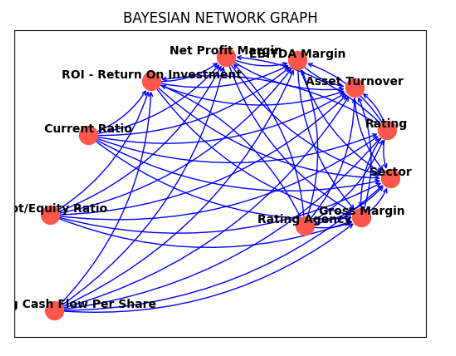
\includegraphics[scale=0.8]{img/bn.png}
\end{figure}
\noindent Di seguito si riporta l'esempio di una \textit{CPD}:

\begin{figure}[H]
    \centering
    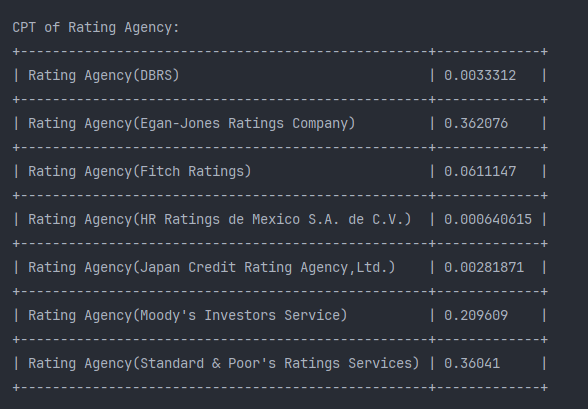
\includegraphics[scale=0.6]{img/cpt.png}
\end{figure}
\noindent Non si è riuscito ad ottenere in tempi ragionevoli la stampa della CPT di una variabile avente dei parents, dato che la rete è molto complessa.

\subsection{Generazione di sample e gestione di dati mancanti}
\noindent Tramite la rete bayesiana è possibile generare nuovi sample, ovvero nuove configurazioni di variabili. Questo è utile per generare nuovi dati da utilizzare per addestrare un modello, o per fare inferenza su nuovi dati.  
\\ Le reti bayesiane sono in grado di gestire casi in cui una variabile di input non è nota. Questo è utile in quanto i dati reali spesso presentano valori mancanti. La rete bayesiana è in grado di fare inferenza su nuovi dati, anche se non tutte le variabili sono note.

\begin{figure}[H]
    \centering
    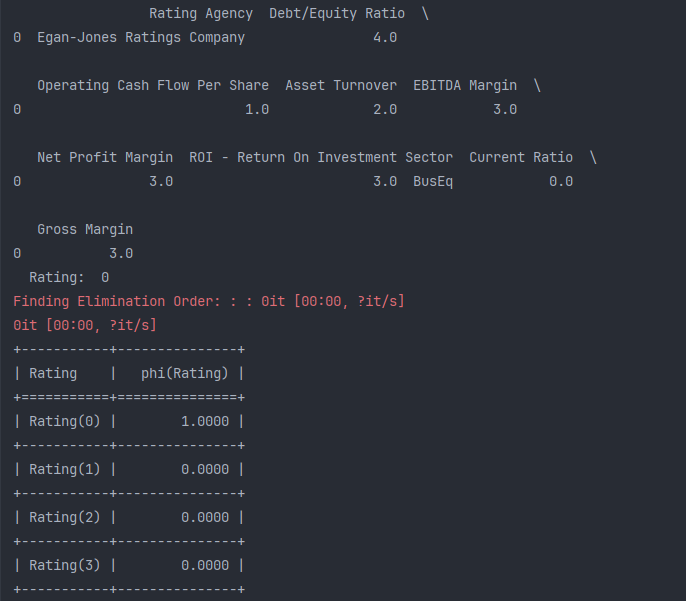
\includegraphics[scale=0.5]{img/sample_generated_bn.png}
    \caption{Esempio generato e classificato}
    \label{fig:normal}
\end{figure}

\begin{figure}[H]
    \centering
    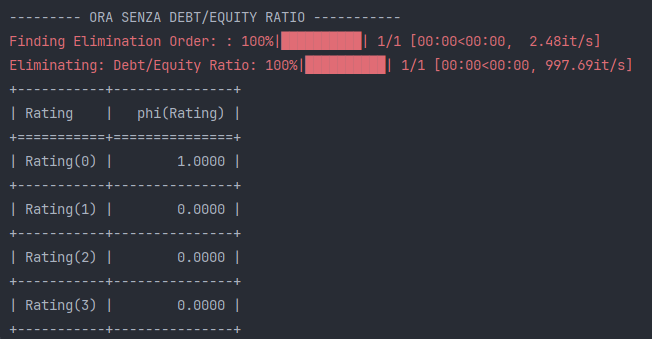
\includegraphics[scale=0.5]{img/sample_generated_bn_without.png}
    \caption{Esempio generato e classificato senza \textit{Debt/Equity Ratio}}
    \label{fig:without}
\end{figure}

\begin{figure}[H]
    \centering
    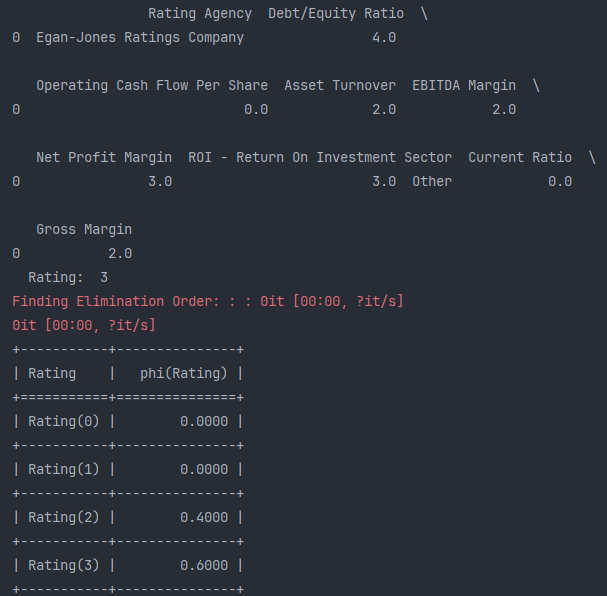
\includegraphics[scale=0.5]{img/so_so.png}
    \caption{Distribuzione di probabilità ampia}
    \label{fig:so}
\end{figure}
\begin{figure}[H]
    \centering
    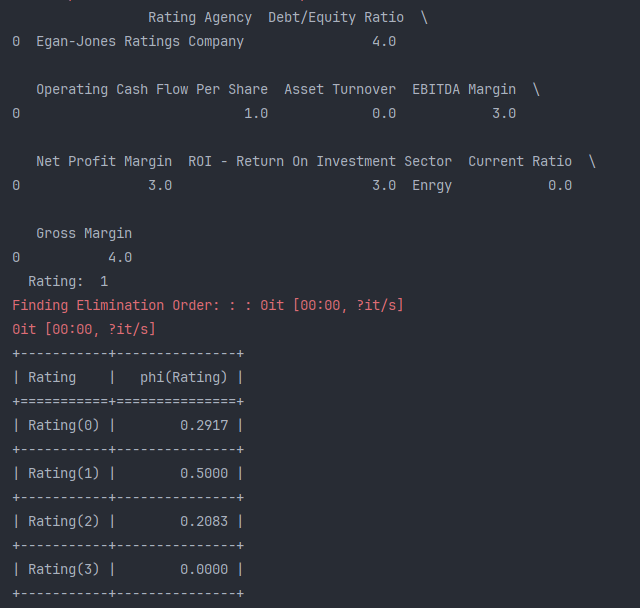
\includegraphics[scale=0.5]{img/bad_prob.png}
    \caption{Distribuzione di probabilità molto ampia}
    \label{fig:bad}
\end{figure}

\noindent Come è possibile notare la rete è in grado di fare inferenza sulla variabile \textit{Rating} anche se non sono note delle variabili, come nel nostro caso di \textit{Debt/Equity Ratio} in $Figura$ \ref{fig:without}.
\\ E' anche possibile notare che non sempre la rete riesce ad assegnare una stima esatta come in $Figura$ \ref{fig:bad}. Alcune volte riesce a stimare una probabilità vicina come in $Figura$ \ref{fig:so}, altre volte invece la distribuzione di probabilità è molto più ampia come in $Figura$ \ref{fig:bad}, riuscendo però comunque a fornire la probabilità più alta alla classe corretta.

\subsection{Valutazione}

\noindent E' possibile stabilire quanto bene il modello descrive i dati osservati. Questo è utile per valutare la bontà del modello. Utilizzeremo il \textit{correlation-score} offerto da \textit{pgmpy}, che effettua un test di correlazione tra le variabili del dataset.\\ Il correlation-score della nostra rete bayesiana rispetto alla sua \textit{balanced accuracy} è circa $0.59$, questo indica che la rete è in grado di catturare una certa correlazione tra le variabili, ma non è in grado di catturare tutte le dipendenze probabilistiche tra le variabili.

\subsection{Query di esempio}
\noindent Le reti bayesiane sono in grado di rispondere a query probabilistiche, ovvero di calcolare la probabilità di una variabile dato un insieme di evidenze. Di seguito si riportano due esempi di query:

\begin{figure}[H]
    \centering
    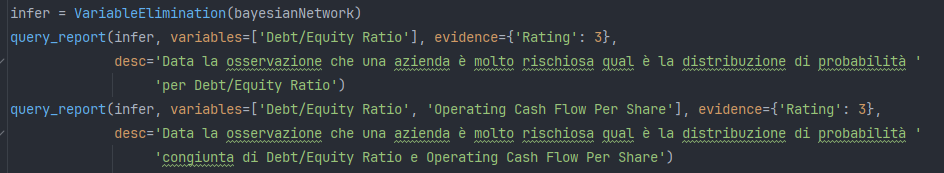
\includegraphics[scale=0.5]{img/ex_query.png}
    \caption{Esempio di query}
\end{figure}

\begin{itemize}[label=-]
    \item Data l'osservazione che una azienda è molto rischiosa qual è la distribuzione di probabilità per \textit{Debt/Equity Ratio}
    \item Data l'osservazione che una azienda è molto rischiosa qual è la distribuzione di probabilità congiunta di \textit{Debt/Equity Ratio} e \textit{Operating Cash Flow Per Share}
\end{itemize}

\begin{figure}[H]
    \centering
    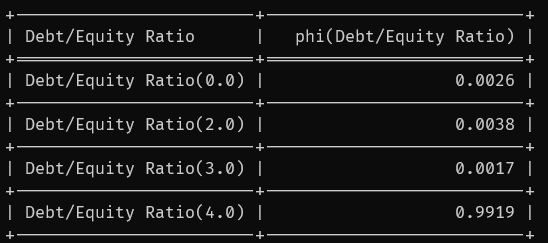
\includegraphics[scale=0.5]{img/firstq.png}
    \caption{Risultato prima query}
\end{figure}

\begin{figure}[H]
    \centering
    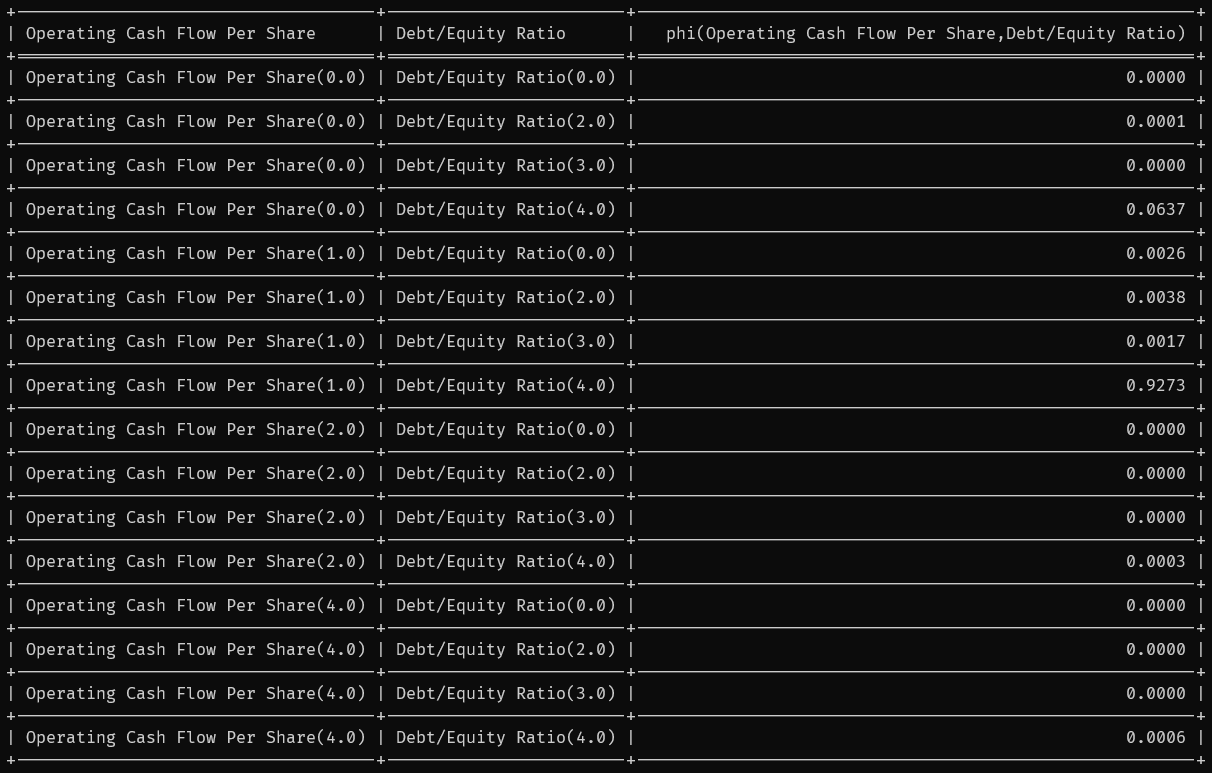
\includegraphics[scale=0.5]{img/secondq.png}
    \caption{Risultato seconda query}
\end{figure}

\noindent Da query di questo tipo possiamo ottenere informazioni utili per trarre delle conclusioni, ad esempio che un'azienda molto rischiosa ha molto probabilmente un \textit{Debt/Equity Ratio} alto, e che quindi tende ad indebitarsi. Dalla seconda query notiamo che se un'azienda è molto rischiosa allora questa ha molto probabilmente un \textit{Debt/Equity Ratio} alto e un \textit{Operating Cash Flow Per Share} basso.

\subsection{Sommario}

\noindent Dato lo sbilanciamento delle classi, e dato il numero minore di esempi su cui è stato allenata la rete bayesiana, dato che eliminando delle feature molti esempi risultavano duplicati, possiamo tutto sommato dire che la rete bayesiana creata ha delle prestazioni accettabili, e permette di eseguire delle query probabilistiche interessanti.
  \newpage
  \section{Conclusioni}
\noindent

\noindent E' stato condotto uno studio sull'applicazione di tecniche di apprendimento supervisionato per classificare il \textit{Corporate Credit Rating} delle aziende. E' stata poi creata una rete bayesiana per fare inferenza su nuovi dati e per rispondere a query probabilistiche. I risultati ottenuti con le varie tecniche sperimentate sono state soddisfacenti, e nonostante la poca quantità di dati a disposizione, la rete bayesiana sembra rappresentare bene il dominio.

\section{Sviluppi futuri}
\noindent Oltre a quelli già proposti, si potrebbero considerare i seguenti sviluppi futuri:
\begin{itemize}[label=-]
    \item Provare a studiare le singole classi originali, avendo a disposizione più dati o con modelli come le reti neurali.
    \item Fare uno studio sul \textit{noise} dei rating, dovuto a fattori esterni da quelli utilizzati
    \item Fare \textit{feature engineering} con altre informazioni del dominio
    \item Fare \textit{feature selection} utilizzando tecniche più avanzate, e quindi non solo basandosi su correlazioni e conoscenza del dominio
    \item Sviluppo di un'interfaccia per poter utilizzare il modello in produzione 
\end{itemize}
  \newpage
  
  \bibliography{bibliography} % Entries are in the bibliography.bib file
\end{document}